\section{Blowup Complex}
\begin{figure*}
\centering
\subfigure[Space and Cover]{
	\label{fig:space-n-cover}
	\def\svgwidth{1.25in}
	\input{figs/blowup_parts.pdf_tex}
}
\hfill
\subfigure[Local pieces of the blowup complex.]{
	\label{fig:local-pieces}
	\def\svgwidth{1.1in}
	\input{figs/local_pieces.pdf_tex}
}
\hfill
\subfigure[The blowup complex.]{
	\label{fig:blowup}
	\def\svgwidth{1.1in}
	\input{figs/blowup_complex.pdf_tex}
}
%\hfill
%\subfigure[Persistence Barcode. Colors represent homology groups computed
%	   on each piece of the blowup complex. Stacked colors represent 
%  parallelism]{
%	\label{fig:barcode}
%	\def\svgwidth{1.1in}
%	\input{figs/barcode.pdf_tex}
%}
\caption{Our approach. We are given a space equipped with a 
	 cover~\subref{fig:space-n-cover}, the former represented by a path with
         four vertices and three edges and the latter represented by ovals.  
	 First, at time $(t = 0)$ we blowup up the space into 
	 local pieces~\subref{fig:local-pieces}, each local piece is a copy of 
	 the corresponding cover set, then, at $(t = 1)$ we glue together 
	 duplicated simplices by adding in the blowup cells, rendering them 
	 homologically equivalent, which gives us the blowup 
	 complex~\subref{fig:blowup}.
}
\label{fig:vignette}
\end{figure*}

In the previous section we introduced the \mv spectral sequence as a tool for computing homology.
While it is straightforward to write down an algorithm for this spectral sequence, it can be at first, a bit challenging to keep track of all the relevant data. In this section we introduce the \mvb, an associated topological space, whose $d$ cells generate $\bigoplus_{i+j = d} E^0_{i,j}$. Studying this gadget is equivalent to studying the spectral sequence, and, we argue, is more intuitive.

Like homology, the blowup complex may be defined for arbitrary topological 
spaces~\cite{zc-lh-08}. However, we focus on blowups of simplicial 
complexes. For a longer exposition of the \mvb{} we refer the reader to Zomorodian
\& Carlsson~\cite{zc-lh-08}. Given a simplicial complex $K$ and cover 
$\C = \{\C_i\}_i$ of $n$ subcomplexes, let 
$\K^J = \bigcap_{k \in J} \C_k$. The \emph{Mayer-Vietoris blowup complex} is:
\begin{linenomath*}
\begin{align*}
\K^\C &= \bigcup_{\emptyset \not = J \subseteq [n-1]} \K^J \times \Delta^J,
\end{align*}
\end{linenomath*}
where $\times$ is the Cartesian product~\cite{zc-lh-08} and $\Delta^J$ is a face of $\N(\C)$. 

 % Do example here before any further talk.
\begin{example}
\label{ex:blowup}
Suppose we have a space $\K$ with cover $\C = \{ \C_0, \C_1 \}$ as is shown on 
the top of Figure~(\ref{fig:space-n-cover}), where we use a line as a 
representative space and ovals to indicate cover sets, and the four vertices
of the line are labeled from left to right as $a, b, c, d$ respectively.
The cover defines the intersection $\K^{[1]} = \K^{ \{ 0 , 1 \} }$. 
The corresponding blowup is shown in in Figure~(\ref{fig:blowup}). We list each of
the relevant pieces of $\K^{\C}$ as well as the nerve of the cover where we denote simplices as strings for 
brevity.  
\begin{linenomath*}
\begin{align*}
\N(\C) &= \{ 0, 1, 01 \} \\
\K^0 \times \Delta^{\{0\}} &= \{a,b,c,ab,bc\} \times \{0\}, \\
\K^1 \times \Delta^{\{1\}} &= \{b,c,d,bc,bd\} \times \{0\}, \\
\K^{[1]} \times \Delta^{[1]} &=\{b,c,bc\} \times \{01\}. 
\end{align*}
\end{linenomath*}
\end{example}

% simplicial
While we may then triangulate the blowup complex to get a simplicial complex in order 
to compute its homology, this is computationally prohibitive, due to the need for triangulation. 
Luckily this approach is also not necessary. To compute the homology of the blowup complex, we may interpret the definition 
above in another way.  At the space level, we may view each cell of the blowup complex as a product 
of two simplices $\sigma \times \tau$, where $\sigma \in \K$ and $\tau \in \N(\C) \subseteq \Delta^{[n]}$.  
For example, the product of two edges, $bc \times 01$, gives us a quadrilateral cell in Example~\ref{ex:blowup}.  
That is the blowup complex is an example of a cellular complex. 
\begin{lemma}
$\K^\C$ is a CW-Complex
\end{lemma}
\begin{proof}
Recall from Lemma~\ref{lem:simp-is-cw} that any simplicial complex is a CW-complex. By Lemma~\ref{lem:cw-complex-product}, $\K^\C$ is a subset of the CW-complex: $\K \times \Delta^{\card{\C}}$. We need to only verify that it is closed. If $\sigma \times \tau \in \K^\C$. Then $\sigma \in \cap_{v \in \tau} \C_{v}$ So therefore $\sigma \in \cap_{v \in \rho} \C_v$ for any $\rho \subset \tau$, so all faces $\sigma \times \rho$ for $\rho$ a face of $\tau$ are contained in $\K^\C$. Since each cover set is closed if $\alpha$ is a face of $\sigma$ then $\alpha \times \tau \in \K^\C$. So therefore $\K^\C$ is a CW-Complex.
\end{proof}

% key property
Our work is based on the following key property; the blowup complex $\K^\C$ has the same homology as its base complex $\K$ in any 
dimension.
\begin{theorem}
If $\K$ is a simplicial complex and $\C$ is any cover by subcomplexes then
\[ H_d(\K^\C) \cong H_d(\K)\] for any $d \geq 0$.
\end{theorem}
\begin{proof}
The original proof is due to Segal~\cite{segal}, where covers are prescribed by open sets. However, in our setting covers are closed sets. To resolve this technicality we invoke this theorem on an open cover $\C'$ of the space $\K'$, the barycentric subdivision of $\K$. The cover $\C' = \{\C'_i\}$ where \[ \C'_i = \bigcup_{v \in \C_i, \textrm{a vertex}} \operatorname{St(v)}. \] Observe that $\K$ is homotopy equivalent to $\K'$ and that $\C_J$, is a deformation retract of $\C'_J$ for any subset $J \subseteq [\card{C}]$.
The latter holds since the operator $\operatorname{St}(\_)$ commutes with intersection, and any set is a deformation retract of its open star. 
Therefore there is a homotopy equivalence between $\C'_J \times \Delta^J$ and $\C_J \times \Delta^J$ for each $J \subset \Delta^n$. Therefore we have that $\K'^{\C'}$ and $\K$ are homotopy equivalent. It remains to show that $\K^\C$ and $\K'^{\C'}$ produce the same homology in each dimension. 

Define $\K_i = \bigcup_{\sigma \in \Delta^n, \dim{\sigma} \leq i} \C_\sigma \times \sigma$ and similarly for $\K'_i$. Observe that  we have already shown that $\K_0$ is homotopy equivalent to $\K'_0$ because we have produced a homotopy equivalence on each element of the disjoint union. Now assume that for any fixed $d > 0$ we have shown the result for all $i < d$. We have the following diagram,
\[ \begin{tikzcd}
\ldots \arrow{r} & H_*(\K'_{d-1}) \arrow{r} & H_*(\K'_d) \arrow{r} & H_*(\K'_d, \K'_{d-1}) \arrow{r} & \ldots \\
\ldots \arrow{r} & H_*(\K_{d-1}) \arrow{r}\arrow{u} & H_*(\K_d) \arrow{r}\arrow{u} & H_*(\K_d, \K_{d-1})\arrow{u}  \arrow{r} & \ldots
\end{tikzcd} \]
where the rows are exact. However, by induction the leftmost and rightmost vertical maps are isomorphisms, and so the middle map must be both surjective and injective, and as such an isomorphism.
\end{proof}
Our approach then is to compute the cellular homology of the blowup complex 
instead of the simplicial homology of base complex. The blowup complex has a structure that allows 
for computation in parallel, unlike the base complex. 

We now examine the chain complex attached to the blowup complex.
% chain
A basis for $C_n(\K^\C)$ is the set composed of elements 
$\sigma \tensor \Delta^J$ for all $\emptyset \not = J \subseteq [n-1]$ and 
simplices $\sigma \in K^J$ where $\dim{\sigma} + \dim{\Delta^J} = n$.  The notation
$\tensor$ denotes \emph{tensor product}. Recall that the tensor product of two 
vector spaces is obtained by taking a quotient of the free vector space
on the cartesian product~\cite[\textrm{Page }218]{hatcher}.
We define the boundary operator as~\cite[\textrm{Lemma }4]{zc-lh-08}:
\begin{linenomath*}
\begin{align*}
\bd{\left (\sigma \tensor \Delta^J \right)}
&=
\bd{\sigma} \tensor \Delta^J + 
(-1)^{\dim{\sigma}}\sigma \tensor \bd\Delta^J.
\end{align*}
\end{linenomath*}
Here, we are defining a boundary operator for the blowup complex on the left 
using the boundary operators on the right, all of which are simplicial and were 
defined in the previous section. 
\begin{example}
The boundary of the quadrilateral cell 
$bc \tensor 01$: in Example~\ref{ex:blowup} is:
\begin{linenomath*}
\begin{align*}
\bd{\left (bc \tensor 01 \right)}
&=
\bd{(bc)} \tensor 01 - bc \tensor \bd(01) \\
&= c \tensor 01 - b \tensor 01 - bc \tensor 1 + bc \tensor 0.
\end{align*}
\end{linenomath*}
\end{example}
Having specified the basis for the chain complex and a boundary operator of 
the blowup complex, we now can compute the homology of the blowup complex. In the next section we
outline how to do this in parallel.

\section{Parallel Homology}
Observe that if we construct a filtration of the blowup complex by increasing nerve dimension, we have a special case of the spectral sequence of the filtration from Section~\ref{sec:ss-filt}. 

%%algorithms figure
\begin{figure}
\centering
\begin{codebox}
\Procname{$\proc{Multicore-Homology}(\K,p)$}
 \li  $\C \gets \proc{Cover}(\K, p)$
 \li  $\K^{\C} \gets \proc{Build-Blowup-Complex}(\K, \C)$
 \li  $\Parfor$   $\Delta^J \in \N(\C)$
 \li  \Do $\proc{Pair-Cells}(\K^{J} \times \Delta^{J})\footnotemark$
      \End
\li $\For$ $d > 0$
 \li \Do $\For$ $\Delta^J \in \N(\C)$ a $d$-cell.
 \li  \Do $\proc{Reduce}(\Cl{(\K^{J} \times \Delta^{J})})$ 
\end{codebox}
\caption{Pseudocode for computing the blowup complex and its homology in parallel. $\proc{Cover}$ can be any algorithm for generating a cover of $\K$ by $p$ subspaces. The procedure $\proc{Reduce}$ is any algorithm for reducing the columns of the boundary matrix of the input subspace.}
\label{fig:multicore-code}
\end{figure}

\begin{figure}
\begin{codebox}
\Procname{$\proc{Build-Blowup-Complex}(\K, \C)$}
\li $\K^{\C} \gets \emptyset$
\li $\Parfor$ $\sigma \in \K$
\li \Do $\For$ $\tau \subseteq \C[\sigma]$
\li \Do $\K^{\C} \gets \K^{\C} \cup (\sigma \times \tau)$ 
\end{codebox}
\end{figure}
\footnotetext{When the list of cells given as input to \proc{Pair-Cells} is not a subcomplex computation should be interpreted as relative homology computation by ignoring
elements of the boundary which are not given in the input.}
The algorithm in Figure~(\ref{fig:multicore-code}) shows how to build the blowup complex and compute its homology in parallel. 
The procedure $\proc{Build-Blowup-Complex}$ runs in parallel and has parallel running time $O(2m/p + p)$ where $m = \card{\K^{\C}}$ and $p$ is the number of processors available. In practice $\proc{Build-Blowup-Complex}$ not only produces a blowup complex but also its skeletal filtration.

The size of the blowup complex depends on the cover. In the worst case, all of 
the simplices in a space $\K$ are contained within all $n$ sets of the cover 
$\C$. In this case, for each simplex $\sigma \in \K$ we have a corresponding 
product cell $\sigma \times \Delta^n$, which has $2^n$ faces. That is, the 
blowup complex \emph{blows up} $\K$ to be $2^n$ times larger, thus deserving 
its name. Therefore, it is imperative to find a cover which minimizes blowup.

\section{Covers}
\label{sec:covers}
Given a simplicial complex $\K$, our goal is to compute its homology.  
Our approach, as illustrated in Figure~(\ref{fig:vignette}), is to find a cover, 
build the associated blowup complex, and compute the homology of the blowup complex in 
parallel. We have now explained all the steps of this approach except how to find a cover. 
We begin in Section~\ref{sec:hardness} by identifying 
properties of covers that lead to efficient computation.
We state an optimization problem over covers which 
minimizes the size of the blowup of a complex. We then show that this optimization problem is \NPH{}.  
In Section~\ref{sec:partition-based-covers}, we describe an algorithm 
that generates covers which have a simple structure, and bounded overlap 
based on graph partitions. We end the section by showing how a partition of the 
0-cells of a complex can be lifted to a partition of a filtration on the complex 
which can be used to compute homology in parallel without building the blowup complex.
\subsection{Minimum Blowups}
\label{sec:hardness}
In this section, we formalize the problem of finding covers
that minimize blowup size. We show that this problem is \NPH{}, and its 
decision-variant, \NPC{}.

We seek a cover which does not yield a large blowup complex. 
To quantify blowup, we define the $\emph{blowup factor}$ as the ratio: 
$\factor.$ We search for a cover $\C$ of size $p$ that minimizes the blowup 
factor. Since we intend to compute the homology of each cover set in parallel,
the number of cover sets should be the number $p$ of available 
processors. Finally, each cover set should be approximately the same 
size. There are many ways of modeling this last constraint. 
We model it by enforcing that no cover set should be larger than a fixed fraction
$\alpha$ of the size of the input complex, where $\alpha \in (\frac{1}{p},1)$. 
Putting together all of the desired properties of blowups, we have the following 
optimization problem stated for $p = 2$ and $\alpha \in (\frac{1}{2}, 1)$:
\begin{description}
\addtolength{\itemsep}{-.7\baselineskip}
\item[\textsc{Problem:}]  \ablp 
\item[\textsc{Instance:}] A simplicial complex $K$
\item[\textsc{Goal:}] Find a cover $\C$ of $\K$ with $2$ elements such that: 
\[ \max{\card{\C_i}} \leq \alpha\card{\K} \textrm{ and } \factor \textrm{ is minimized.} \]
\end{description}
Our goal is to show that this problem is $\NPH{}$ and its decision problem variant $\NPC{}$.
For the decision problem variant to be $\NPC{}$ we need to show that $\factor$ may
be evaluated in polynomial time. Recall that $\K^{\C}$ might be exponentially larger than $\K$. 
For covers by two sets we may employ the following lemma.
\begin{lemma}
\label{lem:char-blowup-sol}
Let $\K$ be a complex and let $\C$ be a cover $\K$ 
of size $p > 1$. Suppose that the intersection
of any three sets in $\C$ vanishes. Then
\begin{equation*}
\factor = 1 + 2\frac{\card{I}}{\card{\K}}. 
\end{equation*}
where $I = \bigcup_{i \neq j}{\C_i \cap \C_j}$.
\end{lemma}
\begin{proof}
This follows directly from the product cell definition of $\K^\C$.
\end{proof}
\noindent Now we observe an important necessary condition of optimal solutions to \ablp{}.
\begin{lemma}
\label{lem:blowup-sol-max-simplices}
Given a complex $\K$, let $\C = \{\C_1, \C_2\}$ be an optimal solution of  \ablp{}. Then 
$\C$ is a partition of $\M(\K)$, the maximal cells of $\K$.
\end{lemma}
\begin{proof}
If $\sigma \in \C_i \cap \C_j$ is a maximal cell, then consider the cover
$\C'$ obtained by removing $\sigma$ from the set of larger
cardinality. $\C'$ is certainly a cover satisfying $\alpha$-balance but
by Lemma~\ref{lem:char-blowup-sol} the blowup factor has decreased
which contradicts the optimality of $\C$.
\end{proof}
\noindent Suppose the input to \ablp{} is a graph $G$. In this context, any cover $\C$ of $G$ is a pair of subgraphs $G_1,G_2$.
Lemma~\ref{lem:blowup-sol-max-simplices} tells us that in any optimal solution, the intersection $I = G_1 \cap G_2$ of these two 
subgraphs is a set of vertices. The requirement that $\C$ is a cover implies that $I$ is a vertex separator. In other words,
given a vertex separator of a graph $G$, we may view it as a cover of that graph and vice versa. 
The equivalent problem for vertex separators for any $\alpha \in (\frac{1}{2},1)$  is:
\begin{description}
\addtolength{\itemsep}{-.8\baselineskip}
\item[\textsc{Problem:}]  \avertex{}
\item[\textsc{Instance:}] A graph $G$
\item[\textsc{Goal:}] Find a vertex separator $(V_1,V_2,I)$ of $G$ such that: 
\[ \card{I} \textrm{ is minimized} \textrm{ subject to } \max_i{(\card{V_i} + \card{E_i})} + \card{I} \leq \alpha(\card{V}+\card{E}),  \]
\end{description}
where $E_i$ is the set of edges with at least one endpoint in $V_i$. \avertex{} is \NPH{} for any $\alpha \in (\frac{1}{2},1)$ and its decision problem variant is \NPC{}~\cite{rhl-yaggpis-14}.
\begin{theorem}
For any $\alpha \in (1/2,1)$ the optimization problem \ablp{} is \NPH{} and its decision problem variant \NPC{}.
\end{theorem}
\begin{proof}
\ablp{} and \avertex{} are equivalent when the former is restricted to graph instances.
\end{proof}
This procedure shows us that finding covers of graphs with bounded overlap also identifies partitions of that graph.
In the next section we show how given a complex $\K$ and a partition of its 1-skeleton one can produce a cover of the entire complex with bounded overlap.
\subsection{Partition-Based Covers}
\begin{figure*}
\centering
\begin{subfigure}[b]{.24\textwidth}
%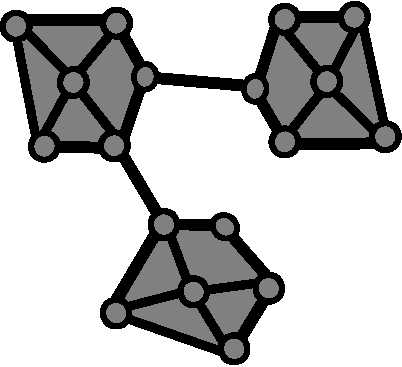
\includegraphics[width=\textwidth]{input_space}
\begin{tikzpicture}[scale=.5,y=-0.80pt, x=0.8pt]
\begin{scope}
\begin{scope}% layer1
    \draw[fill=gray, draw=black,  line width=2]  (142,195) node (a) {} circle (6pt);
    \draw[fill=gray, draw=black,  line width=2]  (95,202) node (b) {} circle (6pt); 
    \draw[fill=gray, draw=black,  line width=2]  (122,155) node (c) {} circle (6pt);  
    \draw[fill=gray, draw=black,  line width=2]  (160,152) node (d) {} circle (6pt);  
     \draw[fill=gray, draw=black,  line width=2]  (170,225)node (e) {}  circle (6pt);  
      \draw[fill=gray, draw=black,  line width=2]  (185,185) node (f) {} circle (6pt);  
      \begin{pgfonlayer}{quadcell}
     \filldraw[color=gray]  (b.center) -- (c.center) -- (d.center) -- (f.center) --  (e.center) -- cycle;
     \end{pgfonlayer}
      \begin{pgfonlayer}{edges}
      \path[color=black, line width=2] (a.center) edge (b.center);
      \path[color=black, line width=2] (a.center) edge (c.center);
      \path[color=black, line width=2] (a.center) edge (d.center);
      \path[color=black, line width=2] (a.center) edge (e.center);
      \path[color=black, line width=2] (a.center) edge (f.center);
      \path[color=black, line width=2] (e.center) edge (f.center) edge (b.center);
      \path[color=black, line width=2] (c.center) edge (b.center) edge (d.center);
       \path[color=black, line width=2] (d.center) edge (f.center);
       \path[color=black, line width =2] (122,155) edge (80, 90);
      \end{pgfonlayer}
\end{scope}
    \begin{scope}[shift={(125,284)},rotate=120]
    \draw[fill=gray, draw=black,  line width=2]  (142,195) node (a) {} circle (6pt);
    \draw[fill=gray, draw=black,  line width=2]  (95,202) node (b) {} circle (6pt); 
    \draw[fill=gray, draw=black,  line width=2]  (122,155) node (c) {} circle (6pt);  
    \draw[fill=gray, draw=black,  line width=2]  (160,152) node (d) {} circle (6pt);  
     \draw[fill=gray, draw=black,  line width=2]  (170,225)node (e) {}  circle (6pt);  
      \draw[fill=gray, draw=black,  line width=2]  (185,185) node (f) {} circle (6pt);  
      \begin{pgfonlayer}{quadcell}
     \filldraw[color=gray]  (b.center) -- (c.center) -- (d.center) -- (f.center) --  (e.center) -- cycle;
     \end{pgfonlayer}
      \begin{pgfonlayer}{edges}
      \path[color=black, line width=2] (a.center) edge (b.center);
      \path[color=black, line width=2] (a.center) edge (c.center);
      \path[color=black, line width=2] (a.center) edge (d.center);
      \path[color=black, line width=2] (a.center) edge (e.center);
      \path[color=black, line width=2] (a.center) edge (f.center);
      \path[color=black, line width=2] (e.center) edge (f.center) edge (b.center);
      \path[color=black, line width=2] (c.center) edge (b.center) edge (d.center);
       \path[color=black, line width=2] (d.center) edge (f.center);
          \path[color=black, line width =2] (160, 152) edge (200, 90);
      \end{pgfonlayer}
                \end{scope}
        \begin{scope}[shift={(198,-138)},rotate=-70]
    \draw[fill=gray, draw=black,  line width=2]  (142,195) node (a) {} circle (6pt);
    \draw[fill=gray, draw=black,  line width=2]  (95,202) node (b) {} circle (6pt); 
    \draw[fill=gray, draw=black,  line width=2]  (122,155) node (c) {} circle (6pt);  
    \draw[fill=gray, draw=black,  line width=2]  (160,152) node (d) {} circle (6pt);  
     \draw[fill=gray, draw=black,  line width=2]  (170,225)node (e) {}  circle (6pt);  
      \draw[fill=gray, draw=black,  line width=2]  (185,185) node (f) {} circle (6pt);  
      \begin{pgfonlayer}{quadcell}
     \filldraw[color=gray]  (b.center) -- (c.center) -- (d.center) -- (f.center) --  (e.center) -- cycle;
     \end{pgfonlayer}
           \begin{pgfonlayer}{edges}
      \path[color=black, line width=2] (a.center) edge (b.center);
      \path[color=black, line width=2] (a.center) edge (c.center);
      \path[color=black, line width=2] (a.center) edge (d.center);
      \path[color=black, line width=2] (a.center) edge (e.center);
      \path[color=black, line width=2] (a.center) edge (f.center);
      \path[color=black, line width=2] (e.center) edge (f.center) edge (b.center);
      \path[color=black, line width=2] (c.center) edge (b.center) edge (d.center);
       \path[color=black, line width=2] (d.center) edge (f.center);
      \end{pgfonlayer}
         \end{scope}
  \end{scope}
\end{tikzpicture}
\caption{Input Complex $\K$}
\label{fig:input}
\end{subfigure}
\hfill
\begin{subfigure}[b]{.24\textwidth}
\begin{tikzpicture}[scale=.5,y=-0.80pt, x=0.8pt]
\begin{scope}% layer1
    \draw[fill=afrapurple, draw=black,  line width=1]  (142,195) node (a) {} circle (6pt);
    \draw[fill=afrapurple, draw=black,  line width=1]  (95,202) node (b) {} circle (6pt); 
    \draw[fill=afrapurple, draw=black,  line width=1]  (122,155) node (c) {} circle (6pt);  
    \draw[fill=afrapurple, draw=black,  line width=1]  (160,152) node (d) {} circle (6pt);  
     \draw[fill=afrapurple, draw=black,  line width=1]  (170,225)node (e) {}  circle (6pt);  
      \draw[fill=afrapurple, draw=black,  line width=1]  (185,185) node (f) {} circle (6pt);  
    \begin{scope}% g10596
      % path7778
      \path[draw=afrapurplelight,line join=miter,line cap=butt,miter limit=4.00,line
        width=2] (142.8068,141.8195) .. controls (140.5229,140.7866) and
        (138.2447,139.7410) .. (135.9724,138.6829) .. controls (133.0686,137.3306) and
        (130.1306,135.9436) .. (126.9750,135.3928) .. controls (123.2061,134.7350) and
        (119.2405,135.3312) .. (115.7977,137.0000) .. controls (112.3550,138.6687) and
        (109.4446,141.3929) .. (107.4859,144.6794) .. controls (105.5194,147.9789) and
        (104.5226,151.7563) .. (103.6919,155.5065) .. controls (102.8612,159.2568) and
        (102.1647,163.0652) .. (100.7192,166.6240) .. controls (98.5492,171.9661) and
        (94.7943,176.4976) .. (90.9055,180.7549) .. controls (87.1005,184.9204) and
        (83.0614,188.9825) .. (80.3662,193.9388) .. controls (79.0186,196.4170) and
        (78.0238,199.1093) .. (77.6619,201.9068) .. controls (77.2999,204.7044) and
        (77.5891,207.6123) .. (78.7040,210.2036) .. controls (79.9202,213.0305) and
        (82.0576,215.3721) .. (84.4182,217.3464) .. controls (89.4627,221.5653) and
        (95.5940,224.2926) .. (101.8472,226.3281) .. controls (108.1004,228.3635) and
        (114.5437,229.7569) .. (120.8468,231.6321) .. controls (125.8989,233.1351) and
        (130.8532,234.9453) .. (135.8468,236.6321) .. controls (143.5496,239.2340) and
        (151.4656,241.5630) .. (159.5933,241.7724) .. controls (167.7210,241.9818) and
        (176.1768,239.8661) .. (182.2754,234.4893) .. controls (186.9397,230.3769) and
        (189.9191,224.6670) .. (192.0037,218.8085) .. controls (194.0883,212.9500) and
        (195.3761,206.8390) .. (197.2754,200.9178) .. controls (198.3603,197.5357) and
        (199.6460,194.2112) .. (200.4716,190.7566) .. controls (201.2972,187.3020) and
        (201.6504,183.6634) .. (200.8468,180.2036) .. controls (200.0756,176.8833) and
        (198.2661,173.8691) .. (196.0175,171.3074) .. controls (193.7689,168.7456) and
        (191.0857,166.6035) .. (188.3386,164.5855) .. controls (182.8445,160.5494) and
        (176.8474,156.7588) .. (173.3140,150.9287) .. controls (171.6874,148.2446) and
        (170.6556,145.2291) .. (168.9715,142.5808) .. controls (168.1294,141.2566) and
        (167.1180,140.0232) .. (165.8705,139.0712) .. controls (164.6230,138.1193) and
        (163.1264,137.4584) .. (161.5611,137.3464) .. controls (160.3978,137.2632) and
        (159.2270,137.4826) .. (158.1251,137.8650) .. controls (157.0233,138.2474) and
        (155.9841,138.7900) .. (154.9709,139.3678) .. controls (152.9447,140.5234) and
        (150.9545,141.8488) .. (148.6798,142.3654) .. controls (146.7303,142.8081) and
        (144.6414,142.6140) .. (142.8068,141.8195);
    \end{scope}
        
    \begin{scope}[shift={(125,284)},rotate=120]
    \draw[fill=afragreen,draw=black,  line width=1]  (142,195) node (a) {} circle (6pt);
    \draw[fill=afragreen, draw=black,  line width=1]  (95,202) node (b) {} circle (6pt); 
    \draw[fill=afragreen, draw=black,  line width=1]  (122,155) node (c) {} circle (6pt);  
    \draw[fill=afragreen, draw=black,  line width=1]  (160,152) node (d) {} circle (6pt);  
     \draw[fill=afragreen, draw=black,  line width=1]  (170,225)node (e) {}  circle (6pt);  
      \draw[fill=afragreen, draw=black,  line width=1]  (185,185) node (f) {} circle (6pt);  
                \end{scope}
    \begin{scope}% g10596
      % path7778
            % path7778-9
      \path[draw=afragreenlight,line join=miter,line cap=butt,miter limit=4.00,line
        width=2] (192.9926,11.9341) .. controls (188.8896,12.6152) and
        (184.9965,14.4282) .. (181.7524,17.0311) .. controls (178.5084,19.6340) and
        (175.9104,23.0138) .. (174.1113,26.7637) .. controls (169.8923,35.5570) and
        (170.1687,45.8307) .. (167.1178,55.0943) .. controls (165.7925,59.1182) and
        (163.8223,63.0319) .. (163.6387,67.2645) .. controls (163.5263,69.8555) and
        (164.1014,72.4453) .. (165.0598,74.8551) .. controls (166.0182,77.2650) and
        (167.3530,79.5081) .. (168.7982,81.6615) .. controls (171.6886,85.9684) and
        (175.0752,90.0199) .. (177.0385,94.8209) .. controls (177.8932,96.9111) and
        (178.4609,99.1056) .. (179.1934,101.2417) .. controls (179.9259,103.3778) and
        (180.8444,105.4903) .. (182.2959,107.2203) .. controls (183.6446,108.8277) and
        (185.4163,110.0510) .. (187.3327,110.9055) .. controls (189.2491,111.7601) and
        (191.3102,112.2567) .. (193.3884,112.5466) .. controls (197.5448,113.1264) and
        (201.7732,112.8927) .. (205.9513,113.2866) .. controls (211.2015,113.7817) and
        (216.3028,115.2594) .. (221.4846,116.2387) .. controls (229.3108,117.7177) and
        (237.3906,118.0536) .. (245.2523,116.7765) .. controls (253.1139,115.4994) and
        (260.7551,112.5790) .. (267.2111,107.9146) .. controls (272.7152,103.9381) and
        (277.3945,98.5796) .. (279.6336,92.1691) .. controls (280.7532,88.9639) and
        (281.2461,85.5266) .. (280.9380,82.1454) .. controls (280.6298,78.7643) and
        (279.5090,75.4439) .. (277.5935,72.6407) .. controls (274.9928,68.8349) and
        (271.0961,66.1511) .. (267.3573,63.4550) .. controls (263.6185,60.7588) and
        (259.8383,57.8362) .. (257.6523,53.7779) .. controls (255.1375,49.1092) and
        (255.0539,43.5530) .. (255.1757,38.2515) .. controls (255.2975,32.9500) and
        (255.5337,27.4624) .. (253.5453,22.5464) .. controls (252.0356,18.8141) and
        (249.2746,15.6239) .. (245.8724,13.4712) .. controls (242.4702,11.3185) and
        (238.4491,10.1936) .. (234.4237,10.1225) .. controls (228.1091,10.0111) and
        (222.0000,12.4065) .. (215.6949,12.7688) .. controls (208.1147,13.2044) and
        (200.4828,10.6908) .. (192.9926,11.9341);
    \end{scope}
        \begin{scope}[shift={(198,-138)},rotate=-70]
    \draw[fill=afrablue, draw=black,  line width=1]  (142,195) node (a) {} circle (6pt);
    \draw[fill=afrablue,draw=black,  line width=1]  (95,202) node (b) {} circle (6pt); 
    \draw[fill=afrablue, draw=black,  line width=1]  (122,155) node (c) {} circle (6pt);  
    \draw[fill=afrablue, draw=black,  line width=1]  (160,152) node (d) {} circle (6pt);  
     \draw[fill=afrablue, draw=black,  line width=1]  (170,225)node (e) {}  circle (6pt);  
      \draw[fill=afrablue, draw=black,  line width=1]  (185,185) node (f) {} circle (6pt);  
         \end{scope}
    \begin{scope}% g10596
      % path7778-4
      \path[draw=afrabluedark,line join=miter,line cap=butt,miter limit=4.00,line
        width=2] (114.2167,41.2393) .. controls (111.5795,35.7883) and
        (110.3171,29.7694) .. (107.8770,24.2274) .. controls (106.6569,21.4563) and
        (105.1297,18.7930) .. (103.0913,16.5543) .. controls (101.0528,14.3156) and
        (98.4767,12.5121) .. (95.5673,11.6741) .. controls (93.1997,10.9921) and
        (90.6823,10.9636) .. (88.2376,11.2700) .. controls (85.7928,11.5764) and
        (83.4024,12.2091) .. (81.0192,12.8346) .. controls (78.6361,13.4602) and
        (76.2421,14.0821) .. (73.7946,14.3663) .. controls (71.3472,14.6505) and
        (68.8282,14.5876) .. (66.4734,13.8627) .. controls (64.2730,13.1855) and
        (62.2883,11.9568) .. (60.3633,10.6941) .. controls (58.4383,9.4313) and
        (56.5283,8.1123) .. (54.4053,7.2216) .. controls (51.6098,6.0489) and
        (48.5082,5.6617) .. (45.4923,5.9694) .. controls (42.4764,6.2771) and
        (39.5466,7.2678) .. (36.8902,8.7284) .. controls (31.5772,11.6495) and
        (27.4415,16.3672) .. (24.2232,21.5057) .. controls (22.6382,24.0364) and
        (21.2430,26.7025) .. (20.3036,29.5370) .. controls (18.2838,35.6312) and
        (18.4521,42.2521) .. (19.4464,48.5949) .. controls (20.4406,54.9377) and
        (22.2309,61.1289) .. (23.4110,67.4398) .. controls (24.3531,72.4776) and
        (24.9041,77.5791) .. (25.4838,82.6714) .. controls (26.3970,90.6930) and
        (27.4212,98.8460) .. (30.7141,106.2174) .. controls (32.3605,109.9031) and
        (34.5756,113.3615) .. (37.4426,116.2032) .. controls (40.3097,119.0448) and
        (43.8461,121.2553) .. (47.7398,122.3203) .. controls (53.5513,123.9098) and
        (59.7541,122.8914) .. (65.5662,121.3043) .. controls (71.3782,119.7172) and
        (77.0782,117.5626) .. (83.0613,116.8547) .. controls (86.5271,116.4447) and
        (90.0380,116.5279) .. (93.5015,116.0988) .. controls (96.9650,115.6697) and
        (100.4817,114.6656) .. (103.1342,112.3975) .. controls (104.6594,111.0933) and
        (105.8396,109.4167) .. (106.7141,107.6106) .. controls (107.5886,105.8044) and
        (108.1667,103.8674) .. (108.6010,101.9082) .. controls (109.4697,97.9899) and
        (109.7788,93.9469) .. (110.9329,90.1030) .. controls (112.5367,84.7609) and
        (115.6923,80.0478) .. (118.3166,75.1262) .. controls (119.6288,72.6653) and
        (120.8193,70.1251) .. (121.6073,67.4499) .. controls (122.3953,64.7747) and
        (122.7732,61.9521) .. (122.4431,59.1829) .. controls (122.0511,55.8942) and
        (120.6821,52.7996) .. (119.0883,49.8963) .. controls (117.4945,46.9930) and
        (115.6592,44.2207) .. (114.2167,41.2393);
    \end{scope}
  \end{scope}
\end{tikzpicture}
\caption{Partition $P$}
\label{fig:part}
\end{subfigure}
\hfill
\begin{subfigure}[b]{.24\textwidth}
\begin{tikzpicture}[scale=.5,y=-0.80pt, x=0.8pt]
\begin{scope}

\begin{scope}% layer1
    \draw[fill=afrapurple, draw=afrapurpledark,  line width=2]  (142,195) node (a) {} circle (6pt);
    \draw[fill=afrapurple, draw=afrapurpledark,  line width=2]  (95,202) node (b) {} circle (6pt); 
    \draw[fill=afrapurple, draw=afrapurpledark,  line width=2]  (122,155) node (c) {} circle (6pt);  
    \draw[fill=afrapurple, draw=afrapurpledark,  line width=2]  (160,152) node (d) {} circle (6pt);  
     \draw[fill=afrapurple, draw=afrapurpledark,  line width=2]  (170,225)node (e) {}  circle (6pt);  
      \draw[fill=afrapurple, draw=afrapurpledark,  line width=2]  (185,185) node (f) {} circle (6pt);  
      \begin{pgfonlayer}{quadcell}
     \filldraw[color=afrapurple]  (b.center) -- (c.center) -- (d.center) -- (f.center) --  (e.center) -- cycle;
     \end{pgfonlayer}
      \begin{pgfonlayer}{edges}
      \path[color=afrapurpledark, line width=2] (a.center) edge (b.center);
      \path[color=afrapurpledark, line width=2] (a.center) edge (c.center);
      \path[color=afrapurpledark, line width=2] (a.center) edge (d.center);
      \path[color=afrapurpledark, line width=2] (a.center) edge (e.center);
      \path[color=afrapurpledark, line width=2] (a.center) edge (f.center);
      \path[color=afrapurpledark, line width=2] (e.center) edge (f.center) edge (b.center);
      \path[color=afrapurpledark, line width=2] (c.center) edge (b.center) edge (d.center);
       \path[color=afrapurpledark, line width=2] (d.center) edge (f.center);
       \path[color=gray, line width =2] (122,155) edge (80, 90);
      \end{pgfonlayer}
    \begin{scope}% g10596
      % path7778
      \path[draw=afrapurplelight,line join=miter,line cap=butt,miter limit=4.00,line
        width=2] (142.8068,141.8195) .. controls (140.5229,140.7866) and
        (138.2447,139.7410) .. (135.9724,138.6829) .. controls (133.0686,137.3306) and
        (130.1306,135.9436) .. (126.9750,135.3928) .. controls (123.2061,134.7350) and
        (119.2405,135.3312) .. (115.7977,137.0000) .. controls (112.3550,138.6687) and
        (109.4446,141.3929) .. (107.4859,144.6794) .. controls (105.5194,147.9789) and
        (104.5226,151.7563) .. (103.6919,155.5065) .. controls (102.8612,159.2568) and
        (102.1647,163.0652) .. (100.7192,166.6240) .. controls (98.5492,171.9661) and
        (94.7943,176.4976) .. (90.9055,180.7549) .. controls (87.1005,184.9204) and
        (83.0614,188.9825) .. (80.3662,193.9388) .. controls (79.0186,196.4170) and
        (78.0238,199.1093) .. (77.6619,201.9068) .. controls (77.2999,204.7044) and
        (77.5891,207.6123) .. (78.7040,210.2036) .. controls (79.9202,213.0305) and
        (82.0576,215.3721) .. (84.4182,217.3464) .. controls (89.4627,221.5653) and
        (95.5940,224.2926) .. (101.8472,226.3281) .. controls (108.1004,228.3635) and
        (114.5437,229.7569) .. (120.8468,231.6321) .. controls (125.8989,233.1351) and
        (130.8532,234.9453) .. (135.8468,236.6321) .. controls (143.5496,239.2340) and
        (151.4656,241.5630) .. (159.5933,241.7724) .. controls (167.7210,241.9818) and
        (176.1768,239.8661) .. (182.2754,234.4893) .. controls (186.9397,230.3769) and
        (189.9191,224.6670) .. (192.0037,218.8085) .. controls (194.0883,212.9500) and
        (195.3761,206.8390) .. (197.2754,200.9178) .. controls (198.3603,197.5357) and
        (199.6460,194.2112) .. (200.4716,190.7566) .. controls (201.2972,187.3020) and
        (201.6504,183.6634) .. (200.8468,180.2036) .. controls (200.0756,176.8833) and
        (198.2661,173.8691) .. (196.0175,171.3074) .. controls (193.7689,168.7456) and
        (191.0857,166.6035) .. (188.3386,164.5855) .. controls (182.8445,160.5494) and
        (176.8474,156.7588) .. (173.3140,150.9287) .. controls (171.6874,148.2446) and
        (170.6556,145.2291) .. (168.9715,142.5808) .. controls (168.1294,141.2566) and
        (167.1180,140.0232) .. (165.8705,139.0712) .. controls (164.6230,138.1193) and
        (163.1264,137.4584) .. (161.5611,137.3464) .. controls (160.3978,137.2632) and
        (159.2270,137.4826) .. (158.1251,137.8650) .. controls (157.0233,138.2474) and
        (155.9841,138.7900) .. (154.9709,139.3678) .. controls (152.9447,140.5234) and
        (150.9545,141.8488) .. (148.6798,142.3654) .. controls (146.7303,142.8081) and
        (144.6414,142.6140) .. (142.8068,141.8195);
    \end{scope}
        \end{scope}
        
    \begin{scope}[shift={(125,284)},rotate=120]
    \draw[fill=afragreen, draw=afragreendark,  line width=2]  (142,195) node (a) {} circle (6pt);
    \draw[fill=afragreen, draw=afragreendark,  line width=2]  (95,202) node (b) {} circle (6pt); 
    \draw[fill=afragreen, draw=afragreendark,  line width=2]  (122,155) node (c) {} circle (6pt);  
    \draw[fill=afragreen, draw=afragreendark,  line width=2]  (160,152) node (d) {} circle (6pt);  
     \draw[fill=afragreen, draw=afragreendark,  line width=2]  (170,225)node (e) {}  circle (6pt);  
      \draw[fill=afragreen, draw=afragreendark,  line width=2]  (185,185) node (f) {} circle (6pt);  
      \begin{pgfonlayer}{quadcell}
     \filldraw[color=afragreen]  (b.center) -- (c.center) -- (d.center) -- (f.center) --  (e.center) -- cycle;
     \end{pgfonlayer}
      \begin{pgfonlayer}{edges}
      \path[color=afragreendark, line width=2] (a.center) edge (b.center);
      \path[color=afragreendark, line width=2] (a.center) edge (c.center);
      \path[color=afragreendark, line width=2] (a.center) edge (d.center);
      \path[color=afragreendark, line width=2] (a.center) edge (e.center);
      \path[color=afragreendark, line width=2] (a.center) edge (f.center);
      \path[color=afragreendark, line width=2] (e.center) edge (f.center) edge (b.center);
      \path[color=afragreendark, line width=2] (c.center) edge (b.center) edge (d.center);
       \path[color=afragreendark, line width=2] (d.center) edge (f.center);
          \path[color=gray, line width =2] (160, 152) edge (200, 90);
      \end{pgfonlayer}
                \end{scope}
    \begin{scope}% g10596
      % path7778
            % path7778-9
      \path[draw=afragreenlight,line join=miter,line cap=butt,miter limit=4.00,line
        width=2] (192.9926,11.9341) .. controls (188.8896,12.6152) and
        (184.9965,14.4282) .. (181.7524,17.0311) .. controls (178.5084,19.6340) and
        (175.9104,23.0138) .. (174.1113,26.7637) .. controls (169.8923,35.5570) and
        (170.1687,45.8307) .. (167.1178,55.0943) .. controls (165.7925,59.1182) and
        (163.8223,63.0319) .. (163.6387,67.2645) .. controls (163.5263,69.8555) and
        (164.1014,72.4453) .. (165.0598,74.8551) .. controls (166.0182,77.2650) and
        (167.3530,79.5081) .. (168.7982,81.6615) .. controls (171.6886,85.9684) and
        (175.0752,90.0199) .. (177.0385,94.8209) .. controls (177.8932,96.9111) and
        (178.4609,99.1056) .. (179.1934,101.2417) .. controls (179.9259,103.3778) and
        (180.8444,105.4903) .. (182.2959,107.2203) .. controls (183.6446,108.8277) and
        (185.4163,110.0510) .. (187.3327,110.9055) .. controls (189.2491,111.7601) and
        (191.3102,112.2567) .. (193.3884,112.5466) .. controls (197.5448,113.1264) and
        (201.7732,112.8927) .. (205.9513,113.2866) .. controls (211.2015,113.7817) and
        (216.3028,115.2594) .. (221.4846,116.2387) .. controls (229.3108,117.7177) and
        (237.3906,118.0536) .. (245.2523,116.7765) .. controls (253.1139,115.4994) and
        (260.7551,112.5790) .. (267.2111,107.9146) .. controls (272.7152,103.9381) and
        (277.3945,98.5796) .. (279.6336,92.1691) .. controls (280.7532,88.9639) and
        (281.2461,85.5266) .. (280.9380,82.1454) .. controls (280.6298,78.7643) and
        (279.5090,75.4439) .. (277.5935,72.6407) .. controls (274.9928,68.8349) and
        (271.0961,66.1511) .. (267.3573,63.4550) .. controls (263.6185,60.7588) and
        (259.8383,57.8362) .. (257.6523,53.7779) .. controls (255.1375,49.1092) and
        (255.0539,43.5530) .. (255.1757,38.2515) .. controls (255.2975,32.9500) and
        (255.5337,27.4624) .. (253.5453,22.5464) .. controls (252.0356,18.8141) and
        (249.2746,15.6239) .. (245.8724,13.4712) .. controls (242.4702,11.3185) and
        (238.4491,10.1936) .. (234.4237,10.1225) .. controls (228.1091,10.0111) and
        (222.0000,12.4065) .. (215.6949,12.7688) .. controls (208.1147,13.2044) and
        (200.4828,10.6908) .. (192.9926,11.9341);
    \end{scope}
        \begin{scope}[shift={(198,-138)},rotate=-70]
    \draw[fill=afrablue, draw=afrabluedark,  line width=2]  (142,195) node (a) {} circle (6pt);
    \draw[fill=afrablue, draw=afrabluedark,  line width=2]  (95,202) node (b) {} circle (6pt); 
    \draw[fill=afrablue, draw=afrabluedark,  line width=2]  (122,155) node (c) {} circle (6pt);  
    \draw[fill=afrablue, draw=afrabluedark,  line width=2]  (160,152) node (d) {} circle (6pt);  
     \draw[fill=afrablue, draw=afrabluedark,  line width=2]  (170,225)node (e) {}  circle (6pt);  
      \draw[fill=afrablue, draw=afrabluedark,  line width=2]  (185,185) node (f) {} circle (6pt);  
      \begin{pgfonlayer}{quadcell}
     \filldraw[color=afrablue]  (b.center) -- (c.center) -- (d.center) -- (f.center) --  (e.center) -- cycle;
     \end{pgfonlayer}
           \begin{pgfonlayer}{edges}
      \path[color=afrabluedark, line width=2] (a.center) edge (b.center);
      \path[color=afrabluedark, line width=2] (a.center) edge (c.center);
      \path[color=afrabluedark, line width=2] (a.center) edge (d.center);
      \path[color=afrabluedark, line width=2] (a.center) edge (e.center);
      \path[color=afrabluedark, line width=2] (a.center) edge (f.center);
      \path[color=afrabluedark, line width=2] (e.center) edge (f.center) edge (b.center);
      \path[color=afrabluedark, line width=2] (c.center) edge (b.center) edge (d.center);
       \path[color=afrabluedark, line width=2] (d.center) edge (f.center);
      \end{pgfonlayer}
         \end{scope}
    \begin{scope}% g10596
      % path7778-4
      \path[draw=afrabluedark,line join=miter,line cap=butt,miter limit=4.00,line
        width=2] (114.2167,41.2393) .. controls (111.5795,35.7883) and
        (110.3171,29.7694) .. (107.8770,24.2274) .. controls (106.6569,21.4563) and
        (105.1297,18.7930) .. (103.0913,16.5543) .. controls (101.0528,14.3156) and
        (98.4767,12.5121) .. (95.5673,11.6741) .. controls (93.1997,10.9921) and
        (90.6823,10.9636) .. (88.2376,11.2700) .. controls (85.7928,11.5764) and
        (83.4024,12.2091) .. (81.0192,12.8346) .. controls (78.6361,13.4602) and
        (76.2421,14.0821) .. (73.7946,14.3663) .. controls (71.3472,14.6505) and
        (68.8282,14.5876) .. (66.4734,13.8627) .. controls (64.2730,13.1855) and
        (62.2883,11.9568) .. (60.3633,10.6941) .. controls (58.4383,9.4313) and
        (56.5283,8.1123) .. (54.4053,7.2216) .. controls (51.6098,6.0489) and
        (48.5082,5.6617) .. (45.4923,5.9694) .. controls (42.4764,6.2771) and
        (39.5466,7.2678) .. (36.8902,8.7284) .. controls (31.5772,11.6495) and
        (27.4415,16.3672) .. (24.2232,21.5057) .. controls (22.6382,24.0364) and
        (21.2430,26.7025) .. (20.3036,29.5370) .. controls (18.2838,35.6312) and
        (18.4521,42.2521) .. (19.4464,48.5949) .. controls (20.4406,54.9377) and
        (22.2309,61.1289) .. (23.4110,67.4398) .. controls (24.3531,72.4776) and
        (24.9041,77.5791) .. (25.4838,82.6714) .. controls (26.3970,90.6930) and
        (27.4212,98.8460) .. (30.7141,106.2174) .. controls (32.3605,109.9031) and
        (34.5756,113.3615) .. (37.4426,116.2032) .. controls (40.3097,119.0448) and
        (43.8461,121.2553) .. (47.7398,122.3203) .. controls (53.5513,123.9098) and
        (59.7541,122.8914) .. (65.5662,121.3043) .. controls (71.3782,119.7172) and
        (77.0782,117.5626) .. (83.0613,116.8547) .. controls (86.5271,116.4447) and
        (90.0380,116.5279) .. (93.5015,116.0988) .. controls (96.9650,115.6697) and
        (100.4817,114.6656) .. (103.1342,112.3975) .. controls (104.6594,111.0933) and
        (105.8396,109.4167) .. (106.7141,107.6106) .. controls (107.5886,105.8044) and
        (108.1667,103.8674) .. (108.6010,101.9082) .. controls (109.4697,97.9899) and
        (109.7788,93.9469) .. (110.9329,90.1030) .. controls (112.5367,84.7609) and
        (115.6923,80.0478) .. (118.3166,75.1262) .. controls (119.6288,72.6653) and
        (120.8193,70.1251) .. (121.6073,67.4499) .. controls (122.3953,64.7747) and
        (122.7732,61.9521) .. (122.4431,59.1829) .. controls (122.0511,55.8942) and
        (120.6821,52.7996) .. (119.0883,49.8963) .. controls (117.4945,46.9930) and
        (115.6592,44.2207) .. (114.2167,41.2393);
    \end{scope}
  \end{scope}
\end{tikzpicture}
\caption{Open Cover $\tilde{\C}$}
\label{fig:cover}
\end{subfigure}
\hfill
\begin{subfigure}[b]{.24\textwidth}
\begin{tikzpicture}[scale=.5,y=-0.80pt, x=0.8pt]
\begin{scope}

\begin{scope}% layer1
    \draw[fill=afrapurple, draw=afrapurpledark,  line width=2]  (142,195) node (a) {} circle (6pt);
    \draw[fill=afrapurple, draw=afrapurpledark,  line width=2]  (95,202) node (b) {} circle (6pt); 
    \draw[fill=afrapurple, draw=afrapurpledark,  line width=2]  (122,155) node (c) {} circle (6pt);  
    \draw[fill=afrapurple, draw=afrapurpledark,  line width=2]  (160,152) node (d) {} circle (6pt);  
     \draw[fill=afrapurple, draw=afrapurpledark,  line width=2]  (170,225)node (e) {}  circle (6pt);  
      \draw[fill=afrapurple, draw=afrapurpledark,  line width=2]  (185,185) node (f) {} circle (6pt);  
      \begin{pgfonlayer}{quadcell}
     \filldraw[color=afrapurple]  (b.center) -- (c.center) -- (d.center) -- (f.center) --  (e.center) -- cycle;
     \end{pgfonlayer}
      \begin{pgfonlayer}{edges}
      \path[color=afrapurpledark, line width=2] (a.center) edge (b.center);
      \path[color=afrapurpledark, line width=2] (a.center) edge (c.center);
      \path[color=afrapurpledark, line width=2] (a.center) edge (d.center);
      \path[color=afrapurpledark, line width=2] (a.center) edge (e.center);
      \path[color=afrapurpledark, line width=2] (a.center) edge (f.center);
      \path[color=afrapurpledark, line width=2] (e.center) edge (f.center) edge (b.center);
      \path[color=afrapurpledark, line width=2] (c.center) edge (b.center) edge (d.center);
       \path[color=afrapurpledark, line width=2] (d.center) edge (f.center);
       \path[color=gray, line width =2] (122,155) edge (80, 90);
      \end{pgfonlayer}
    \begin{scope}% g10596
      % path7778
      \path[draw=afrapurplelight,line join=miter,line cap=butt,miter limit=4.00,line
        width=2] (142.8068,141.8195) .. controls (140.5229,140.7866) and
        (138.2447,139.7410) .. (135.9724,138.6829) .. controls (133.0686,137.3306) and
        (130.1306,135.9436) .. (126.9750,135.3928) .. controls (123.2061,134.7350) and
        (119.2405,135.3312) .. (115.7977,137.0000) .. controls (112.3550,138.6687) and
        (109.4446,141.3929) .. (107.4859,144.6794) .. controls (105.5194,147.9789) and
        (104.5226,151.7563) .. (103.6919,155.5065) .. controls (102.8612,159.2568) and
        (102.1647,163.0652) .. (100.7192,166.6240) .. controls (98.5492,171.9661) and
        (94.7943,176.4976) .. (90.9055,180.7549) .. controls (87.1005,184.9204) and
        (83.0614,188.9825) .. (80.3662,193.9388) .. controls (79.0186,196.4170) and
        (78.0238,199.1093) .. (77.6619,201.9068) .. controls (77.2999,204.7044) and
        (77.5891,207.6123) .. (78.7040,210.2036) .. controls (79.9202,213.0305) and
        (82.0576,215.3721) .. (84.4182,217.3464) .. controls (89.4627,221.5653) and
        (95.5940,224.2926) .. (101.8472,226.3281) .. controls (108.1004,228.3635) and
        (114.5437,229.7569) .. (120.8468,231.6321) .. controls (125.8989,233.1351) and
        (130.8532,234.9453) .. (135.8468,236.6321) .. controls (143.5496,239.2340) and
        (151.4656,241.5630) .. (159.5933,241.7724) .. controls (167.7210,241.9818) and
        (176.1768,239.8661) .. (182.2754,234.4893) .. controls (186.9397,230.3769) and
        (189.9191,224.6670) .. (192.0037,218.8085) .. controls (194.0883,212.9500) and
        (195.3761,206.8390) .. (197.2754,200.9178) .. controls (198.3603,197.5357) and
        (199.6460,194.2112) .. (200.4716,190.7566) .. controls (201.2972,187.3020) and
        (201.6504,183.6634) .. (200.8468,180.2036) .. controls (200.0756,176.8833) and
        (198.2661,173.8691) .. (196.0175,171.3074) .. controls (193.7689,168.7456) and
        (191.0857,166.6035) .. (188.3386,164.5855) .. controls (182.8445,160.5494) and
        (176.8474,156.7588) .. (173.3140,150.9287) .. controls (171.6874,148.2446) and
        (170.6556,145.2291) .. (168.9715,142.5808) .. controls (168.1294,141.2566) and
        (167.1180,140.0232) .. (165.8705,139.0712) .. controls (164.6230,138.1193) and
        (163.1264,137.4584) .. (161.5611,137.3464) .. controls (160.3978,137.2632) and
        (159.2270,137.4826) .. (158.1251,137.8650) .. controls (157.0233,138.2474) and
        (155.9841,138.7900) .. (154.9709,139.3678) .. controls (152.9447,140.5234) and
        (150.9545,141.8488) .. (148.6798,142.3654) .. controls (146.7303,142.8081) and
        (144.6414,142.6140) .. (142.8068,141.8195);
    \end{scope}
        \end{scope}
        
    \begin{scope}[shift={(125,284)},rotate=120]
    \draw[fill=afragreen, draw=afragreendark,  line width=2]  (142,195) node (a) {} circle (6pt);
    \draw[fill=afragreen, draw=afragreendark,  line width=2]  (95,202) node (b) {} circle (6pt); 
    \draw[fill=afragreen, draw=afragreendark,  line width=2]  (122,155) node (c) {} circle (6pt);  
    \draw[fill=afragreen, draw=afragreendark,  line width=2]  (160,152) node (d) {} circle (6pt);  
     \draw[fill=afragreen, draw=afragreendark,  line width=2]  (170,225)node (e) {}  circle (6pt);  
      \draw[fill=afragreen, draw=afragreendark,  line width=2]  (185,185) node (f) {} circle (6pt);  
      \begin{pgfonlayer}{quadcell}
     \filldraw[color=afragreen]  (b.center) -- (c.center) -- (d.center) -- (f.center) --  (e.center) -- cycle;
     \end{pgfonlayer}
      \begin{pgfonlayer}{edges}
      \path[color=afragreendark, line width=2] (a.center) edge (b.center);
      \path[color=afragreendark, line width=2] (a.center) edge (c.center);
      \path[color=afragreendark, line width=2] (a.center) edge (d.center);
      \path[color=afragreendark, line width=2] (a.center) edge (e.center);
      \path[color=afragreendark, line width=2] (a.center) edge (f.center);
      \path[color=afragreendark, line width=2] (e.center) edge (f.center) edge (b.center);
      \path[color=afragreendark, line width=2] (c.center) edge (b.center) edge (d.center);
       \path[color=afragreendark, line width=2] (d.center) edge (f.center);
          \path[color=gray, line width =2] (160, 152) edge (200, 90);
      \end{pgfonlayer}
                \end{scope}
    \begin{scope}% g10596
      % path7778
            % path7778-9
      \path[draw=afragreenlight,line join=miter,line cap=butt,miter limit=4.00,line
        width=2] (192.9926,11.9341) .. controls (188.8896,12.6152) and
        (184.9965,14.4282) .. (181.7524,17.0311) .. controls (178.5084,19.6340) and
        (175.9104,23.0138) .. (174.1113,26.7637) .. controls (169.8923,35.5570) and
        (170.1687,45.8307) .. (167.1178,55.0943) .. controls (165.7925,59.1182) and
        (163.8223,63.0319) .. (163.6387,67.2645) .. controls (163.5263,69.8555) and
        (164.1014,72.4453) .. (165.0598,74.8551) .. controls (166.0182,77.2650) and
        (167.3530,79.5081) .. (168.7982,81.6615) .. controls (171.6886,85.9684) and
        (175.0752,90.0199) .. (177.0385,94.8209) .. controls (177.8932,96.9111) and
        (178.4609,99.1056) .. (179.1934,101.2417) .. controls (179.9259,103.3778) and
        (180.8444,105.4903) .. (182.2959,107.2203) .. controls (183.6446,108.8277) and
        (185.4163,110.0510) .. (187.3327,110.9055) .. controls (189.2491,111.7601) and
        (191.3102,112.2567) .. (193.3884,112.5466) .. controls (197.5448,113.1264) and
        (201.7732,112.8927) .. (205.9513,113.2866) .. controls (211.2015,113.7817) and
        (216.3028,115.2594) .. (221.4846,116.2387) .. controls (229.3108,117.7177) and
        (237.3906,118.0536) .. (245.2523,116.7765) .. controls (253.1139,115.4994) and
        (260.7551,112.5790) .. (267.2111,107.9146) .. controls (272.7152,103.9381) and
        (277.3945,98.5796) .. (279.6336,92.1691) .. controls (280.7532,88.9639) and
        (281.2461,85.5266) .. (280.9380,82.1454) .. controls (280.6298,78.7643) and
        (279.5090,75.4439) .. (277.5935,72.6407) .. controls (274.9928,68.8349) and
        (271.0961,66.1511) .. (267.3573,63.4550) .. controls (263.6185,60.7588) and
        (259.8383,57.8362) .. (257.6523,53.7779) .. controls (255.1375,49.1092) and
        (255.0539,43.5530) .. (255.1757,38.2515) .. controls (255.2975,32.9500) and
        (255.5337,27.4624) .. (253.5453,22.5464) .. controls (252.0356,18.8141) and
        (249.2746,15.6239) .. (245.8724,13.4712) .. controls (242.4702,11.3185) and
        (238.4491,10.1936) .. (234.4237,10.1225) .. controls (228.1091,10.0111) and
        (222.0000,12.4065) .. (215.6949,12.7688) .. controls (208.1147,13.2044) and
        (200.4828,10.6908) .. (192.9926,11.9341);
    \end{scope}
    
        \begin{scope}[shift={(198,-138)},rotate=-70]
    \draw[fill=afrablue, draw=afrabluedark,  line width=2]  (142,195) node (a) {} circle (6pt);
    \draw[fill=afrablue, draw=afrabluedark,  line width=2]  (95,202) node (b) {} circle (6pt); 
    \draw[fill=afrablue, draw=afrabluedark,  line width=2]  (122,155) node (c) {} circle (6pt);  
    \draw[fill=afrablue, draw=afrabluedark,  line width=2]  (160,152) node (d) {} circle (6pt);  
     \draw[fill=afrablue, draw=afrabluedark,  line width=2]  (170,225)node (e) {}  circle (6pt);  
      \draw[fill=afrablue, draw=afrabluedark,  line width=2]  (185,185) node (f) {} circle (6pt);  
      \begin{pgfonlayer}{quadcell}
     \filldraw[color=afrablue]  (b.center) -- (c.center) -- (d.center) -- (f.center) --  (e.center) -- cycle;
     \end{pgfonlayer}
           \begin{pgfonlayer}{edges}
      \path[color=afrabluedark, line width=2] (a.center) edge (b.center);
      \path[color=afrabluedark, line width=2] (a.center) edge (c.center);
      \path[color=afrabluedark, line width=2] (a.center) edge (d.center);
      \path[color=afrabluedark, line width=2] (a.center) edge (e.center);
      \path[color=afrabluedark, line width=2] (a.center) edge (f.center);
      \path[color=afrabluedark, line width=2] (e.center) edge (f.center) edge (b.center);
      \path[color=afrabluedark, line width=2] (c.center) edge (b.center) edge (d.center);
       \path[color=afrabluedark, line width=2] (d.center) edge (f.center);
      \end{pgfonlayer}
         \end{scope}
    \begin{scope}% g10596
      % path7778-4
      \path[draw=afrabluedark,line join=miter,line cap=butt,miter limit=4.00,line
        width=2] (114.2167,41.2393) .. controls (111.5795,35.7883) and
        (110.3171,29.7694) .. (107.8770,24.2274) .. controls (106.6569,21.4563) and
        (105.1297,18.7930) .. (103.0913,16.5543) .. controls (101.0528,14.3156) and
        (98.4767,12.5121) .. (95.5673,11.6741) .. controls (93.1997,10.9921) and
        (90.6823,10.9636) .. (88.2376,11.2700) .. controls (85.7928,11.5764) and
        (83.4024,12.2091) .. (81.0192,12.8346) .. controls (78.6361,13.4602) and
        (76.2421,14.0821) .. (73.7946,14.3663) .. controls (71.3472,14.6505) and
        (68.8282,14.5876) .. (66.4734,13.8627) .. controls (64.2730,13.1855) and
        (62.2883,11.9568) .. (60.3633,10.6941) .. controls (58.4383,9.4313) and
        (56.5283,8.1123) .. (54.4053,7.2216) .. controls (51.6098,6.0489) and
        (48.5082,5.6617) .. (45.4923,5.9694) .. controls (42.4764,6.2771) and
        (39.5466,7.2678) .. (36.8902,8.7284) .. controls (31.5772,11.6495) and
        (27.4415,16.3672) .. (24.2232,21.5057) .. controls (22.6382,24.0364) and
        (21.2430,26.7025) .. (20.3036,29.5370) .. controls (18.2838,35.6312) and
        (18.4521,42.2521) .. (19.4464,48.5949) .. controls (20.4406,54.9377) and
        (22.2309,61.1289) .. (23.4110,67.4398) .. controls (24.3531,72.4776) and
        (24.9041,77.5791) .. (25.4838,82.6714) .. controls (26.3970,90.6930) and
        (27.4212,98.8460) .. (30.7141,106.2174) .. controls (32.3605,109.9031) and
        (34.5756,113.3615) .. (37.4426,116.2032) .. controls (40.3097,119.0448) and
        (43.8461,121.2553) .. (47.7398,122.3203) .. controls (53.5513,123.9098) and
        (59.7541,122.8914) .. (65.5662,121.3043) .. controls (71.3782,119.7172) and
        (77.0782,117.5626) .. (83.0613,116.8547) .. controls (86.5271,116.4447) and
        (90.0380,116.5279) .. (93.5015,116.0988) .. controls (96.9650,115.6697) and
        (100.4817,114.6656) .. (103.1342,112.3975) .. controls (104.6594,111.0933) and
        (105.8396,109.4167) .. (106.7141,107.6106) .. controls (107.5886,105.8044) and
        (108.1667,103.8674) .. (108.6010,101.9082) .. controls (109.4697,97.9899) and
        (109.7788,93.9469) .. (110.9329,90.1030) .. controls (112.5367,84.7609) and
        (115.6923,80.0478) .. (118.3166,75.1262) .. controls (119.6288,72.6653) and
        (120.8193,70.1251) .. (121.6073,67.4499) .. controls (122.3953,64.7747) and
        (122.7732,61.9521) .. (122.4431,59.1829) .. controls (122.0511,55.8942) and
        (120.6821,52.7996) .. (119.0883,49.8963) .. controls (117.4945,46.9930) and
        (115.6592,44.2207) .. (114.2167,41.2393);
    \end{scope}
      % path7778-4-3-2
      \begin{scope}[shift={(-2,0)}]
      \path[draw=gray,line join=miter,line cap=butt,miter limit=4.00,line
        width=2] (114.1034,116.8692) .. controls (111.1695,110.7306) and
        (110.3701,103.6287) .. (106.6867,97.9084) .. controls (103.7047,93.2773) and
        (98.9630,89.8930) .. (93.7303,88.1731) .. controls (89.3756,86.7418) and
        (84.4966,86.4476) .. (80.2729,88.2287) .. controls (78.1610,89.1193) and
        (76.2515,90.5226) .. (74.8644,92.3472) .. controls (73.4774,94.1718) and
        (72.6293,96.4223) .. (72.5850,98.7139) .. controls (72.5275,101.6860) and
        (73.8064,104.5649) .. (75.6275,106.9144) .. controls (77.4486,109.2639) and
        (79.7902,111.1508) .. (82.1520,112.9559) .. controls (86.1024,115.9750) and
        (90.1843,118.8390) .. (93.8684,122.1779) .. controls (97.5524,125.5167) and
        (100.8601,129.3829) .. (102.8860,133.9234) .. controls (105.8553,140.5786) and
        (105.8702,148.1454) .. (107.7720,155.1805) .. controls (108.7229,158.6980) and
        (110.1846,162.1412) .. (112.5528,164.9104) .. controls (114.9211,167.6796) and
        (118.2779,169.7244) .. (121.9122,169.9874) .. controls (125.4114,170.2406) and
        (128.9404,168.7985) .. (131.4675,166.3650) .. controls (133.9946,163.9315) and
        (135.5454,160.5744) .. (136.0554,157.1034) .. controls (136.5654,153.6323) and
        (136.0734,150.0561) .. (134.9295,146.7396) .. controls (133.7856,143.4230) and
        (132.0054,140.3526) .. (129.9392,137.5173) .. controls (124.8166,130.4880) and
        (117.8541,124.7167) .. (114.1034,116.8692);
	\end{scope}
   \begin{scope}[shift={(0,2)}]
      % path7778-4-3-2-1
      \path[draw=gray,line join=miter,line cap=butt,miter limit=4.00,line
        width=2] (142.7047,48.6196) .. controls (135.3135,48.2685) and
        (127.9060,48.3981) .. (120.5141,48.0604) .. controls (115.2209,47.8185) and
        (109.7294,47.3665) .. (104.7924,49.2905) .. controls (102.1093,50.3361) and
        (99.6927,52.0733) .. (97.8842,54.3141) .. controls (96.0756,56.5550) and
        (94.8844,59.2969) .. (94.5282,62.1544) .. controls (94.1721,65.0119) and
        (94.6587,67.9759) .. (95.9525,70.5484) .. controls (97.2464,73.1210) and
        (99.3481,75.2876) .. (101.9024,76.6172) .. controls (104.5040,77.9713) and
        (107.5009,78.4411) .. (110.4319,78.3367) .. controls (113.3629,78.2323) and
        (116.2472,77.5770) .. (119.0709,76.7841) .. controls (123.8544,75.4409) and
        (128.5225,73.6954) .. (133.3440,72.4953) .. controls (138.1655,71.2953) and
        (143.2192,70.6493) .. (148.1054,71.5508) .. controls (155.3659,72.8902) and
        (161.5711,77.4783) .. (168.4951,80.0411) .. controls (171.9571,81.3225) and
        (175.6841,82.0982) .. (179.3461,81.6322) .. controls (181.1771,81.3992) and
        (182.9758,80.8534) .. (184.5876,79.9542) .. controls (186.1995,79.0549) and
        (187.6210,77.7970) .. (188.6404,76.2582) .. controls (190.4795,73.4821) and
        (190.9039,69.8913) .. (190.0864,66.6631) .. controls (189.2689,63.4350) and
        (187.2854,60.5691) .. (184.7698,58.3872) .. controls (179.7384,54.0234) and
        (172.9269,52.4313) .. (166.3655,51.2891) .. controls (158.5410,49.9270) and
        (150.6379,48.9964) .. (142.7047,48.6196);
\end{scope}
  \end{scope}
\end{tikzpicture}
\caption{Cover $U$}
\label{fig:closed-cover}
\end{subfigure}
\caption{Our heuristic algorithm for cover construction. Given 
	the input complex $\K$ shown in~(\subref{fig:input}) we first, partition the vertex
	set of the underlying graph $G$ as shown in~(\subref{fig:part}) then, extend this to
	an open cover $\tilde{\C}$ of $\K$~(\subref{fig:cover}). Finally, we produce, $\C$ a
	cover~(\subref{fig:closed-cover}).}
\label{fig:vignette1}
\end{figure*}

\label{sec:partition-based-covers}
\label{sec:pcover}
\begin{figure}[h!]
\begin{description}
\addtolength{\itemsep}{-.65\baselineskip}
\item[\small\textbf{Input:}] \small A complex $\K$, and a graph partition $P$.
\item[\small\textbf{Output:}] \small A cover $\C$, of size $\card{P}+1$.
\end{description}
\vspace{-.6cm}
\begin{codebox}
\Procname{$\proc{Open-Cover}(\K,P)$}
 \li	$\id{\C} \gets \emptyset$
 \li  \Parfor\,$ \sigma \gets \sigma_1$ \To $\sigma_m \in \K$
 \li 	   \Do  $\id{\C}[\sigma] \gets \proc{Partition-Cell}(P,\sigma)$
          \End
 \li \Return \id{\C}
  \End
\end{codebox}
\caption{The pseudocode for $\proc{Open-Cover}$ which runs in $O(md/p)$ time, where $m$ is the 
number of simplices in $\K$ a $d$-dimensional complex, and $p$ is the 
maximum number of available cores.}
\label{alg:open-cov}
\end{figure}
\begin{figure}[h!]
\begin{description}
\addtolength{\itemsep}{-.65\baselineskip}
\item[\small \textbf{Input:}] \small A graph partition $P$ of size $p$, and simplex $\sigma$
\item[\small \textbf{Output:}] \small The index $i \in [p]$ of  $\tilde{\C}$ to place $\sigma$.
\end{description}
\vspace{-.65cm}
\begin{codebox}
\Procname{$\proc{Partition-Cell}(P, \sigma = [v_0, \ldots, v_d])$}
 \li	$R \gets \emptyset$
 \li  \For $v \gets v_0$ \To $v_d \in \sigma$
 \li 	   \Do $R \gets P(v_0)$
          \End
 \li	\If $\card{R} = 1$ \Return $R[0]$
 \li    \Else \Return $\card{P}$
\end{codebox}
\caption{The pseudocode for $\proc{Partition-Cell}$. $P$ is indexed starting at 0. For a vertex $v$, $P(v)$ 
denotes the index of the partition set of $P$ containing $v$.}
\end{figure}
In this section we describe an algorithm for generating covers on an 
arbitrary complex from a partition of its one skeleton. We emphasize that while we propose a specific
algorithm for generating covers any procedure for generating covers suffices. In many situations there might be a 
better approach for generating covers than the one presented. Recall that in the worst case, a cover may produce an exponentially large blowup. 
However, the heuristic presented in this section guarantees that $\factor < 3$. 

There are many algorithms for generating covers, and they are all valid inputs to our parallel algorithms. 
Zomorodian \& Carlsson consider two methods for cover enumeration, \emph{random $\epsilon$-balls} 
and \emph{tilings} \cite{zc-lh-08}. For complexes embedded in a low dimensional space one might consider
algorithms based on \emph{Voronoi diagrams} or when the data is available by level sets of 
\emph{Morse functions}.  However, in the general setting it is possible to generate a cover of an 
arbitrary simplicial complex from a partition of its one skeleton with a simple intersection pattern.

The algorithm $\proc{Partition-Based-Cover}$, illustrated in Figure~(\ref{fig:vignette1}), takes a complex $\K$ and positive 
integer $p \geq 2$ as input and produces a cover $\C$ of size $p+1$ as output. 
First, we extract the one-skeleton of $\K$ and represent it as a graph $G$. 
Second, we find a graph partition $P$ of $G$ of size $p$.  
Third, we extend $P$ to an open cover $\tilde{\C}$. Finally, we extend $\tilde{\C}$ to a cover $\C$. The algorithms
for producing these two covers are called $\proc{Open-Cover}$ and
$\proc{Close-Cover}$, respectively. 

There are many algorithms for computing partitions of graphs which
seem to fall into four major classes of algorithms: geometric, non-geometric, 
spectral, and hybrid methods \cite{fj-gp-98}. Hybrid methods mix the techniques of the 
other three. In practice, we use \textsc{Metis}, a hybrid method, since it tends to produce balanced partitions quickly~\cite{KaKu95}. 
Of course any partitioning scheme will work. Next, we describe $\proc{Open-Cover}(\K,P)$, which extends a partition of $G$ to an open cover of $\K$. 

The procedure $\proc{Open-Cover}(\K,P)$ is given in Algorithm~\ref{alg:open-cov} and outputs an open cover $\tilde{\C} = \{\tilde{\C}_i\}_{i \in [p]}$ which is a partition of $\K$. Given a partition $P = \{P_i\}_{i \in [p-1]}$ of the vertex set of $G$ we expand $P$ to $\tilde{\C}$. Specifically, we first create sets 
$\tilde{\C} = \{\tilde{\C}_i\}_{i \in [p]}$ where a simplex $\sigma$ is placed into $\tilde{\C}_i$ for $i \in [p-1]$ 
if all of its vertices lie in $P_i$ and is added to $\tilde{\C}_p$ otherwise. 

In the procedure $\proc{Close-Cover}$ we replace $\tilde{\C}_{i}$ with $\C_i = \Cl{(\tilde{\C}_i)}$. However, $\tilde{\C}_i$ is closed for $i \in [p-1]$ by construction so we only close the last set.  Both $\proc{Open-Cover}$ and $\proc{Close-Cover}$ can be implemented in parallel. 
We have the following lemma: 
\begin{lemma}
\label{lem:blowup-factor}
Given a complex $\K$, $p \geq 2$, $\proc{Partition-Based-Cover}(\K, p)$ 
generates a cover $\C$ with $\factor < 3$. 
\end{lemma}
\begin{proof}
For a complex $\K$ and $p \geq 2$ let $\C$ be the cover of $\K$ by $p+1$ subcomplexes output by \proc{Partition-Based-Cover}(\K,p). The first
$p$ cover sets are disjoint since they are formed from disjoint sets of vertices. Therefore there can be at most pairwise intersections.
It follows by Lemma~\ref{lem:char-blowup-sol} that $\factor < 3$.
\end{proof}

Since we are interested only in the homology of $\K$ and not its persistent homology we may avoid the construction of the blowup complex and use the open cover generated to place a filtration on $\K$. In particular, consider the filtration on $\K$ obtained by ordering $\tilde{\C}_i < \tilde{\C}_p$ for $i \in [p-1]$. It is clear that before including $\tilde{\C}_p$ the complex is again disconnected and thus these columns of the matrix may be reduced in parallel. Finally, we reduce this last set of columns against the columns from the first $p$ cover sets. We call this procedure $\proc{Heuristic-MH}$.
 
In the next section we compare these two parallel algorithms against the standard serial algorithm as well as the algorithm $\proc{Chunk}$ of Bauer et. al\@ on a series of examples. The $\proc{Chunk}$ algorithm is based on the spectral sequence of a filtration~\cite{bkr-cccph-13}.
\section{Experiments}
\begin{figure}[h]
\centering
\begin{subfigure}[b]{.45\textwidth}
\centering
\begin{tikzpicture}[scale=.65]
\begin{axis}[xlabel=\# of partitions, minor y tick num={1}, ylabel=speedup factor, legend style={legend pos=north west, font=\small}]
\legend{\multiblob, \bunny, \clique, \gnp, \sphere, ideal}
\addplot table [x=num_partitions, skip coords between index={0}{1}, y=speedup, col sep=comma, ignore chars=']
{pgf-speedup-figs/results/concurrent_homology/clique.11.22720.csv};
\addplot table [x=num_partitions, skip coords between index={0}{1}, y=speedup, col sep=comma, ignore chars=']
{pgf-speedup-figs/results/concurrent_homology/bunny..05.csv};
\addplot table [x=num_partitions, skip coords between index={0}{1}, y=speedup, col sep=comma, ignore chars=']
{pgf-speedup-figs/results/concurrent_homology/clique.20.csv};
\addplot table [x=num_partitions, skip coords between index={0}{1}, y=speedup, col sep=comma, ignore chars=']
{pgf-speedup-figs/results/concurrent_homology/gnp.1250.047.csv};
\addplot table [x=num_partitions, skip coords between index={0}{1}, y=speedup, col sep=comma, ignore chars=']
{pgf-speedup-figs/results/concurrent_homology/sphere.csv};
\addplot[dash pattern=on 4pt off 1pt on 4pt off 4pt, domain=2:10]{x+1};
\end{axis}
\end{tikzpicture}
\caption{Speedup factor for reducing $\partial_{\K^{\C}}$}
\label{fig:blowup-homology-speedup}
\end{subfigure}
\hfill
\begin{subfigure}[b]{.45\textwidth}
\centering
\begin{tikzpicture}[scale=.65]
%\pgfplotsset{ymax=5}
\begin{axis}[xlabel=\# of partitions/threads, minor y tick num={1}, ylabel=speedup factor, legend style={legend pos=north west, font=\small}]
\legend{\multiblob, \bunny, \clique, \gnp, \sphere, ideal}
\addplot table [x=num_partitions, skip coords between index={0}{1}, y=speedup, col sep=comma, ignore chars=']
{pgf-speedup-figs/results/cover_homology/clique.11.22720.csv};
\addplot table [x=num_partitions, skip coords between index={0}{1}, y=speedup, col sep=comma, ignore chars=']
{pgf-speedup-figs/results/cover_homology/bunny..05.csv};
\addplot table [x=num_partitions, skip coords between index={0}{1}, y=speedup, col sep=comma, ignore chars=']
{pgf-speedup-figs/results/cover_homology/clique.20.csv};
\addplot table [x=num_partitions, skip coords between index={0}{1}, y=speedup, col sep=comma, ignore chars=']
{pgf-speedup-figs/results/cover_homology/gnp.1250.047.csv};
\addplot table [x=num_partitions, skip coords between index={0}{1}, y=speedup, col sep=comma, ignore chars=']
{pgf-speedup-figs/results/cover_homology/sphere.csv};
\addplot[dash pattern=on 4pt off 1pt on 4pt off 4pt, domain=2:10]{x};
\end{axis}
\end{tikzpicture}
\caption{Speedup factor for reducing $\partial_{\K}$}
\label{fig:nonblowup-homology-speedup}
\end{subfigure}
\caption{(Left) Speedup factor $T_s/T_p$ where $T_p$ is the time to reduce $\partial_{\K^\C}$ in parallel on $p+1$ threads  and $T_s$ is the time to reduce $\partial_K$ in serial. (Right) Speedup factor of $T_s/T_p$ where $T_p$ measures the time to reduce $\partial_{\K}$ in parallel.}
\label{fig:reduction-speedup}
\end{figure}
\label{sec:exp}
In this section, we describe the implementation of our algorithms
and explore their performance on real and synthetic data. We compare our
performance against our existing serial software as well as the Persistent Homology Algorithm Toolbox (PHAT)~\cite{bkr-cccph-13}. 
Our implementation is in \cplusplus\, using the generic programming paradigm. 
We rely on the METIS library for computing graph partitions 
\cite{KaKu95}, the Intel Threading Building Blocks 
Library~\cite{IntelTBB} for parallelism, and our own
library for homology computation. Our parallel implementation of $\proc{Multicore-Homology}$ computes
an initial filtration on $\K$, a cover $\C$, builds a blowup complex $\K^{\C}$ 
with its associated filtration [in parallel], and then reduces $\partial_{\K^{\C}}$.
For $\proc{Heuristic-MH}$ we reduces a permuted $\partial_\K$, instead of building $\K^{\C}$.
Unlike the pseudo-code for $\proc{Multicore-Homology}$ when reducing $\partial_{\K^{\C}}$,
our implementation reduces the columns corresponding to cells of the form $\sigma \times \tau$ with $\dim{(\tau)} > 0$ in serial
after the parallel reduction of all other cells. Preliminary experiments suggested that
this added parallelism would not produce speedup. Our serial implementation only 
computes an identical initial filtration, and then reduces $\partial_\K$.

We now provide details on how these experiments were carried out.
As previously mentioned all of our experiments are done 
using 11 cores on a 2 CPU, 12 Core, x86-64 Linux Machine, with 2.93 GHz Intel 
Xeon X5670 Processors, 74 GB of RAM, and hyper-threading disabled.
We time both parallel and serial programs in wall-clock time using the tbb::clock. 
We measure the total amount of memory requested by a process, its \emph{resident set size},
via the \emph{process filesystem}. This is an upper bound on the total memory used.  
Each time measured is the \emph{make span} or longest running thread time within a section of code. 
Time is always reported in seconds, and all reported measurements are averaged over 10 trials.
We remind the reader that while we may spawn $p$ threads we only ever have at most $p-1$ of the total $p$ cores 
in order to leave room for system processes. In this work we use at most one thread per available 
core. When running PHAT we used the latest stable version 1.4 and the ``vector vector" option as 
this is the same basic data structure we use in our library. All software was compiled with gcc and optimizations
enabled.

\subsection{Data}
\begin{table*}
  \begin{center}
    \small
    \begin{tabular}{crrrrrrrr}
      \hline
      \multicolumn{6}{c}{Input Statistics} \\
      \multicolumn{1}{c}{$D$} &
      \multicolumn{1}{c}{$\card{D}$} &
      \multicolumn{1}{c}{$\epsilon$, $p$} &
      \multicolumn{1}{c}{$\card{E}$} &
      \multicolumn{1}{c}{$d$} &
      \multicolumn{1}{c}{$\card{\K}$} \\
      \hline
      \blobs &  249,920 & - & 1,272,319 & 10 & 46,530,559 \\
      \clique &  20 & - & 190 & 19 & 1,048,575 \\
      \bunny & 34,837 & 0.05 & 489,876 & 3 & 9,714,912 \\
      \sphere & 50,000 & 0.18 & 546,388 & 8 & 19,134,612 \\
      \gnp & 1250 & 0.047 &  & 4 & 73,309 \\
      \hline
    \end{tabular}
  \end{center}
  \caption{%
    Input Statistics: The name $D$, and number of vertices of each data set $\card{D}$, 
    as well as input parameter $\epsilon$ or $p$ in the case of a random graph, 
    embedding dimension $d = \dim{D}$, size $\card{K}$, and edge-set size $\card{E}$ of each complex $\K$. 
  }
  \label{tab:data}
\end{table*}
 
We summarize each data set in Table~\ref{tab:data}.  All complexes are skeletons of a Vietoris-Rips Complex~\cite{z-fcv-10}.  
Next, we describe the input space for each experiment. 
Recall that {\blobs} is a collection of 22,720 copies of a fully connected 10 dimensional complex on 11 vertices, organized
into 10 groups of 2,272, with each 
copy within a group connected to the next by a single edge, and each group connected to the next by a single edge. 
{\clique} is a fully connected complex on 19 vertices. Recall that $\Delta^{[n]}$ has $\Theta(2^n)$ 
faces. {\bunny} is a 3-complex built on a set of points sampled from the 
\emph{Stanford bunny}. We create {\sphere} by using Muller's method~\cite{m-nmgpuns-59} to sample 
uniformly on the unit 3-sphere and then use the diagonal map
$x \rightarrow (x,x)$ to embed the points in $\R^8$~\cite{hatcher}. {\gnp} is a 
4-dimensional clique complex built on a sparse \Erdos-\Renyi\ graph $G(n,p)$ 
with $n = 1250$ and $p = 0.047$.

\subsection{Statistics}
\begin{figure}
\centering
\begin{subfigure}[b]{.45\textwidth}
\centering
\begin{tikzpicture}[scale=.65]
\begin{axis}[xlabel=\# of partitions, ylabel={$\hat{\alpha}= \max_i \card{P_i} / \card{\K}$}, legend style={legend pos=north east, font=\small}]
\legend{\multiblob, \bunny, \clique, \gnp, \sphere, ideal}
\addplot table [x=num_partitions, y=graph_balance_ratio, col sep=comma] {pgf-speedup-figs/results/concurrent_homology/clique.11.22720.csv};
\addplot table [x=num_partitions, y=graph_balance_ratio, col sep=comma] {pgf-speedup-figs/results/concurrent_homology/bunny..05.csv};
\addplot table [x=num_partitions, y=graph_balance_ratio, col sep=comma] {pgf-speedup-figs/results/concurrent_homology/clique.20.csv};
\addplot table [x=num_partitions, y=graph_balance_ratio, col sep=comma] {pgf-speedup-figs/results/concurrent_homology/gnp.1250.047.csv};
\addplot table [x=num_partitions, y=graph_balance_ratio, col sep=comma] {pgf-speedup-figs/results/concurrent_homology/sphere.csv};
\addplot[dash pattern=on 4pt off 1pt on 4pt off 4pt, domain=2:10]{1/x};
\end{axis}
\end{tikzpicture}
\caption{Partition Balance Ratio $\hat{\alpha}$}
\label{fig:graph-balance}
\end{subfigure}
\begin{subfigure}[b]{.45\textwidth}
\centering
\begin{tikzpicture}[scale=.65]
%\pgfplotsset{ymax=5}
\begin{axis}[xlabel=\# of partitions, ymax=50000, ylabel={\# of edges}, legend style={legend pos=north west, font=\small}]
\legend{\multiblob, \bunny, \clique, \gnp, \sphere, ideal}
\addplot table [x=num_partitions, skip coords between index={0}{1}, y=edgecut, col sep=comma, ignore chars=']
{pgf-speedup-figs/results/concurrent_homology/clique.11.22720.csv};
\addplot table [x=num_partitions, skip coords between index={0}{1}, y=edgecut, col sep=comma, ignore chars=']
{pgf-speedup-figs/results/concurrent_homology/bunny..05.csv};
\addplot table [x=num_partitions, skip coords between index={0}{1}, y=edgecut, col sep=comma, ignore chars=']
{pgf-speedup-figs/results/concurrent_homology/clique.20.csv};
\addplot table [x=num_partitions, skip coords between index={0}{1}, y=edgecut, col sep=comma, ignore chars=']
{pgf-speedup-figs/results/concurrent_homology/gnp.1250.047.csv};
\addplot table [x=num_partitions, skip coords between index={0}{1}, y=edgecut, col sep=comma, ignore chars=']
{pgf-speedup-figs/results/concurrent_homology/sphere.csv};
\end{axis}
\end{tikzpicture}
\caption{Edgecut}
\label{fig:graph-edgecut}
\end{subfigure}
\begin{subfigure}[b]{.45\textwidth}
\centering
\begin{tikzpicture}[scale=.65]
\begin{axis}[xlabel=\# of partitions, ylabel={$\alpha = \max_i \card{\C_i} / \card{\K}$}, legend style={legend pos=north east, font=\small},legend style={at={(.95,.55)},anchor=east}]
\legend{\multiblob, \bunny, \clique, \gnp, \sphere, ideal}
\addplot table [x=num_partitions, y=cover_balance_ratio, col sep=comma,skip coords between index={0}{1}] 
{pgf-speedup-figs/results/concurrent_homology/clique.11.22720.csv};
\addplot table [x=num_partitions, y=cover_balance_ratio, col sep=comma, skip coords between index={0}{1}] 
{pgf-speedup-figs/results/concurrent_homology/bunny..05.csv};
\addplot table [x=num_partitions,skip coords between index={0}{1}, y=cover_balance_ratio, col sep=comma] 
{pgf-speedup-figs/results/concurrent_homology/clique.20.csv};
\addplot table [x=num_partitions, skip coords between index={0}{1},y=cover_balance_ratio, col sep=comma] 
{pgf-speedup-figs/results/concurrent_homology/gnp.1250.047.csv};
\addplot table [x=num_partitions, skip coords between index={0}{1},y=cover_balance_ratio, col sep=comma] 
{pgf-speedup-figs/results/concurrent_homology/sphere.csv};
\addplot[dash pattern=on 4pt off 1pt on 4pt off 4pt, domain=2:10]{1/x};
\end{axis}
\end{tikzpicture}
\caption{Balance Ratio for $\C$}
\label{fig:balance-factors}
\end{subfigure}
\begin{subfigure}[b]{.45\textwidth}
\centering
\begin{tikzpicture}[scale=.65]
\begin{axis}[xlabel=\# of partitions, ylabel=$\ratio$, legend style={legend pos=north east, font=\small},legend style={at={(.95,.55)},anchor=east}]
\legend{\multiblob, \bunny, \clique, \gnp, \sphere, worst case}
\addplot table [x=num_partitions, y=blowup_factor, col sep=comma,skip coords between index={0}{1}] 
{pgf-speedup-figs/results/concurrent_homology/clique.11.22720.csv};
\addplot table [x=num_partitions, y=blowup_factor, col sep=comma, skip coords between index={0}{1}] 
{pgf-speedup-figs/results/concurrent_homology/bunny..05.csv};
\addplot table [x=num_partitions,skip coords between index={0}{1}, y=blowup_factor, col sep=comma] 
{pgf-speedup-figs/results/concurrent_homology/clique.20.csv};
\addplot table [x=num_partitions, skip coords between index={0}{1},y=blowup_factor, col sep=comma] 
{pgf-speedup-figs/results/concurrent_homology/gnp.1250.047.csv};
\addplot table [x=num_partitions, skip coords between index={0}{1},y=blowup_factor, col sep=comma] 
{pgf-speedup-figs/results/concurrent_homology/sphere.csv};
\addplot[dash pattern=on 4pt off 1pt on 4pt off 4pt, domain=2:10]{3};
\end{axis}
\end{tikzpicture}
\caption{Blowup Factor}
\label{fig:blowup-factors}
\end{subfigure}
\caption{Statistics for partitions and covers generated}
\label{fig:statistics}
\end{figure}

Recall from Section~\ref{sec:partition-based-covers} that our input is a complex
$\K$ and integer $p > 1$. Our goal is to build a balanced cover for 
which $\factor$ is as small as possible. First, we build a a graph partition of
the one skeleton $G(\K)$. To produce our graph partition we chose the
unsupervised graph partitioning algorithm METIS because it tends to produce 
balanced graph partitions. In Figure~(\ref{fig:graph-balance}) we show the balance
ratio $\hat{\alpha} = \max_i{\card{V_i}}/\card{V}$ for each partition produced by METIS.
Next, we complete our graph partition into a cover. Figure~(\ref{fig:balance-factors})
shows the balance ratio $\alpha = \max_i{\card{\C_i}}/\card{\K}$ for covers
produced by: $\proc{Partition-Based-Cover}$.
Finally, the procedure $\proc{Build-Blowup-Complex}$ 
computes the blowup complex along with its filtration. 
In Figure~(\ref{fig:blowup-factors}) we plot $\factor$. Recall that 
covers produced by $\proc{Partition-Based-Cover}$ have
$\factor < 3$ and in general for $n$ sets this ratio is at worst $O(2^n)$. 

\subsection{Timing \& Measurements}
For each of our data sets we present the speedup factor of
our reduction algorithm versus serial persistence in Figure~(\ref{fig:reduction-speedup}).

First, we can see that our techniques tend to scale the best on inputs
in which all topological features are localized by the cover. For example, we see the
best performance on $\blobs$. This is not surprising since for any $p \in [2, 10]$ 
this complex exhibits a partition-based cover which balances its 
46.5M simplices nearly perfectly while maintaining that the size of all intersections between all sets is exactly $p-1$.
Second, geometric inputs such as $\bunny$ and $\sphere$ have entirely global topology; These
global topological features are resolved by reducing a handful of columns in the portion of the computation that is 
executed serially. However, these inputs still emit balanced covers, so we see speedup since 
overall the bulk of the work is roughly evenly divided across each core.
Finally, we see that inputs which are flag complexes of cliques or expander graphs, 
such as $\clique$ or $\gnp$, emit no balanced cover and all covers seem to result in a large blowup complex. 
As expected our parallel algorithms exhibit no speedup on these inputs. 
\begin{figure}
\centering
%\fbox{
\begin{tikzpicture}[scale=.65]
\begin{semilogyaxis}[
name=plot1,
%legend pos=outer north east,
xmin=0,
xmax=11,
ymin=1,
ymax=20000,
xlabel=\# of partition sets,
ylabel=Maximum Resident Set Size (MB),
title={$\proc{Multicore-Homology}$},
legend style={at = {(.9,.5)},font=\large}]
%\legend{\multiblob, \bunny, \clique, \gnp, \sphere}
\addplot table [x=num_partitions, y=max memory (MB), col sep=comma] {pgf-speedup-figs/results/concurrent_homology/clique.11.22720.csv};
\addplot table [x=num_partitions, y=max memory (MB), col sep=comma] {pgf-speedup-figs/results/concurrent_homology/bunny..05.csv};
\addplot table [x=num_partitions, y=max memory (MB), col sep=comma] {pgf-speedup-figs/results/concurrent_homology/clique.20.csv};
\addplot table [x=num_partitions, y=max memory (MB), col sep=comma] {pgf-speedup-figs/results/concurrent_homology/gnp.1250.047.csv};
\addplot table [x=num_partitions,, y=max memory (MB), col sep=comma] {pgf-speedup-figs/results/concurrent_homology/sphere.csv};
\end{semilogyaxis}
\begin{semilogyaxis}[
name=plot2,
at=(plot1.outer east), anchor=outer west,
xmin=0,
xmax=11,
ymin=1,
ymax=20000,
xlabel=\# of threads,
title={$\proc{Chunk}$},
legend style={legend pos=south east,font=\tiny}, 
legend style={at = {(1,.45)},font=\large}]
%\legend{\multiblob, \bunny, \clique, \gnp, \sphere}
\addplot table [x=num_threads, y=max memory (MB), col sep=comma] {pgf-speedup-figs/results/phat_14_chunk/clique.11.22720.csv};
\addplot table [x=num_threads, y=max memory (MB), col sep=comma] {pgf-speedup-figs/results/phat_14_chunk/bunny..05.csv};
\addplot table [x=num_threads, y=max memory (MB), col sep=comma] {pgf-speedup-figs/results/phat_14_chunk/clique.20.csv};
\addplot table [x=num_threads, y=max memory (MB), col sep=comma] {pgf-speedup-figs/results/phat_14_chunk/gnp.1250.047.csv};
\addplot table [x=num_threads, y=max memory (MB), col sep=comma] {pgf-speedup-figs/results/phat_14_chunk/sphere.csv};
\end{semilogyaxis}

\begin{semilogyaxis}[
name=plot3,
at=(plot1.below south west), anchor=above north west,
xmax=11,
ymin=1,
ymax=20000,
title={$\proc{Heuristic-MH}$},
xlabel=\# of partition sets, 
legend style={at={(.98,.43)}, font=\footnotesize}]
\legend{\multiblob, \bunny, \clique, \gnp, \sphere}
\addplot table [x=num_partitions, y=max memory (MB), col sep=comma] {pgf-speedup-figs/results/cover_homology/clique.11.22720.csv};
\addplot table [x=num_partitions, y=max memory (MB), col sep=comma] {pgf-speedup-figs/results/cover_homology/bunny..05.csv};
\addplot table [x=num_partitions, y=max memory (MB), col sep=comma] {pgf-speedup-figs/results/cover_homology/clique.20.csv};
\addplot table [x=num_partitions, y=max memory (MB), col sep=comma] {pgf-speedup-figs/results/cover_homology/gnp.1250.047.csv};
\addplot table [x=num_partitions, y=max memory (MB), col sep=comma] {pgf-speedup-figs/results/cover_homology/sphere.csv};
\end{semilogyaxis}

\begin{semilogyaxis}[
name=plot4,
at=(plot3.outer east), anchor=outer west,
ymin=1,
ymax=20000,
xmin=0,
xmax=11,
xlabel= \# of threads, 
title={$\proc{Spectral-Sequence}$},
minor y tick num={5},
legend style={at={(1,.6)}, font=\large}]
\addplot table [x=num_threads, y=max memory (MB), col sep=comma] {pgf-speedup-figs/results/phat_14_ss/clique.11.22720.csv};
\addplot table [x=num_threads, y=max memory (MB), col sep=comma] {pgf-speedup-figs/results/phat_14_ss/bunny..05.csv};
\addplot table [x=num_threads, y=max memory (MB), col sep=comma] {pgf-speedup-figs/results/phat_14_ss/clique.20.csv};
\addplot table [x=num_threads, y=max memory (MB), col sep=comma] {pgf-speedup-figs/results/phat_14_ss/gnp.1250.047.csv};
\addplot table [x=num_threads, y=max memory (MB), col sep=comma] {pgf-speedup-figs/results/phat_14_ss/sphere.csv};
\end{semilogyaxis}
\end{tikzpicture}
\caption{Total memory usage for each algorithm. Recall that PHAT takes as input a boundary matrix whereas the 
procedures outlined in this work take as input a simplicial complex and generates an identical boundary matrix before reducing it. 
At $x=1$ on all plots we display the memory used for the standard algorithm from the appropriate software package.}
\label{fig:memory-usage}
\end{figure}

We observe that with the exception of $\gnp$ the parallel reduction of the boundary matrix for the blowup complex 
runs in time similar to the parallel reduction of the permuted boundary matrix. However there is overhead to each approach. 
Both algorithms require the computation of a cover. On one hand, to reduce $\partial_{\K^\C}$ we must first build $\K^\C$ and its associated filtration. 
However in $\proc{Heuristic-MH}$ we must construct a new filtration on $\K$. 
\begin{figure}
\centering
\begin{subfigure}[b]{.45\textwidth}
\centering
\begin{tikzpicture}[scale=.65]
\begin{axis}[
name=left axis,
ymin=0,
ymax=15,
xmax=12,
xlabel=\# of  partitions,
ylabel=time (seconds),
minor y tick num={5},
legend style={font=\large}]
\legend{\multiblob, \bunny, \clique, \gnp, \sphere, ideal}
\addplot table [x=num_partitions, skip coords between index={0}{1}, y=build_blowup, col sep=comma, ignore chars=']
{pgf-speedup-figs/results/concurrent_homology/clique.11.22720.csv};
\addplot table [x=num_partitions, skip coords between index={0}{1}, y=build_blowup, col sep=comma, ignore chars=']
{pgf-speedup-figs/results/concurrent_homology/bunny..05.csv};
\addplot table [x=num_partitions, skip coords between index={0}{1}, y=build_blowup, col sep=comma, ignore chars=']
{pgf-speedup-figs/results/concurrent_homology/clique.20.csv};
\addplot table [x=num_partitions, skip coords between index={0}{1}, y=build_blowup, col sep=comma, ignore chars=']
{pgf-speedup-figs/results/concurrent_homology/gnp.1250.047.csv};
\addplot table [x=num_partitions, skip coords between index={0}{1}, y=build_blowup, col sep=comma, ignore chars=']
{pgf-speedup-figs/results/concurrent_homology/sphere.csv};
\end{axis}
\end{tikzpicture}
\caption{Time to build $\K^{\C}$ with $p$ partition sets.}
\end{subfigure}
\begin{subfigure}[b]{.45\textwidth}
\centering
\begin{tikzpicture}[scale=.65]
\begin{axis}[
ymin=0,
ymax=15,
xmax=12,
xlabel=\# of  partitions,
%ylabel=time (seconds),
minor y tick num={5},
legend style={legend pos = north west,font=\large}]
%\legend{\multiblob, \bunny, \clique, \gnp, \sphere}
\addplot table [x=num_partitions, skip coords between index={0}{1}, y=re-filter complex, col sep=comma, ignore chars=']
{pgf-speedup-figs/results/cover_homology/clique.11.22720.csv};
\addplot table [x=num_partitions, skip coords between index={0}{1}, y=re-filter complex, col sep=comma, ignore chars=']
{pgf-speedup-figs/results/cover_homology/bunny..05.csv};
\addplot table [x=num_partitions, skip coords between index={0}{1}, y=re-filter complex, col sep=comma, ignore chars=']
{pgf-speedup-figs/results/cover_homology/clique.20.csv};
\addplot table [x=num_partitions, skip coords between index={0}{1}, y=re-filter complex, col sep=comma, ignore chars=']
{pgf-speedup-figs/results/cover_homology/gnp.1250.047.csv};
\addplot table [x=num_partitions, skip coords between index={0}{1}, y=re-filter complex, col sep=comma, ignore chars=']
{pgf-speedup-figs/results/cover_homology/sphere.csv};
\end{axis}
\end{tikzpicture}
\caption{Time to re-filter $\K$}
\end{subfigure}
\caption{Comparison of the time to build a blowup complex in $O(\frac{m}{p} + p)$ time versus time to re-filter the base complex in $O(\frac{m}{p}\log{m})$.}
\label{fig:blowup-vs-no-blowup}
\end{figure}

Recall that the procedure $\proc{Build-Blowup-Complex}$ runs in parallel and has parallel running time $O(2m/p + p)$ time where $m = \card{\K^{\C}}$ 
and $p$ is the number of processors available. 
The procedure $\proc{Build-Blowup-Complex}$ is implemented as a variant of the $\proc{Prefix-Sum}$ algorithm~\cite{breshears}. 
In particular this means that $\proc{Build-Blowup-Complex}$ produces the filtration of the blowup complex along with the complex itself. 
Aside from its output $\proc{Build-Blowup-Complex}$ only uses $O(p)$ extra space. When avoiding the blowup complex we 
do so by creating a new filtration in $O(\frac{m}{p}\log{m})$ where $m = \card{\K}$ and $p$ is the total number of available threads.

Figure~(\ref{fig:blowup-vs-no-blowup}) compares the running time of $\proc{Build-Blowup-Complex}$ against the time to re-filter $\K$.
From the standpoint of memory consumption it is clear that the blowup avoiding algorithm is a better choice. However,
when the resulting blowup complex is similar in size to the original space, It may be possible to significantly improve overall running time 
by building the blowup complex simply because the process of sorting may end up being slower than building the blowup.

We end this section by comparing the \mv algorithm to $\proc{Chunk}$ and \proc{Spectral-Sequence} algorithms available in PHAT.
$\proc{Spectral-Sequence}$ and $\proc{Chunk}$ are parallel implementations of the spectral sequence algorithm based on the spectral sequence of a filtration~\cite{bkr-cccph-13}.s
We plot the time to reduce $\partial_{\K}$ and $\partial_{\K^\C}$ with $p$ threads versus the time for the each algorithm from PHAT to reduce 
$\partial_{\K}$ in Figure~(\ref{fig:ctl_vs_phat}). 
Figure~(\ref{fig:memory-usage}) compares the total memory usage for these algorithms. Recall that PHAT takes as input
a description of $\partial_{\K}$ whereas for our experiments we read in as input $\K$ and then build and reduce $\partial_{\K^{\_}}$. 
While the implementation of the chunk algorithm in PHAT can be significantly faster than its implementation of the standard algorithm,
their algorithms do not always seem to scale with the number of available threads. Our experiments suggest that the algorithms 
provided in PHAT attain speedup mainly due to the out of order nature of their reductions. The two optimizations used
in these algorithms significantly reduces the total work required as compared to the serial algorithm, but these optimizations 
do not seem to help scalability.  Practically, this software is still in the early stages of development, so we expect future versions to 
be more competitive.
\begin{figure}
\centering
\begin{tikzpicture}[scale=.65]
\begin{semilogyaxis}[
name=plot1,
ymin=.09,
ymax=25,
xmin=0,
xmax=12,
xlabel=\# of  threads, 
title={$\proc{Multicore-Homology}$},
ylabel= time to reduce boundary matrix (seconds),
minor y tick num={5},
legend style={at = {(.25,.6)}, font=\large}]
%\legend{\multiblob, \bunny, \clique, \gnp, \sphere}
\addplot table [x=num_threads, y=persistence, col sep=comma] {pgf-speedup-figs/results/concurrent_homology/clique.11.22720.csv};
\addplot table [x=num_threads, y=persistence, col sep=comma] {pgf-speedup-figs/results/concurrent_homology/bunny..05.csv};
\addplot table [x=num_threads, y=persistence, col sep=comma] {pgf-speedup-figs/results/concurrent_homology/clique.20.csv};
\addplot table [x=num_threads, y=persistence, col sep=comma] {pgf-speedup-figs/results/concurrent_homology/gnp.1250.047.csv};
\addplot table [x=num_threads, y=persistence, col sep=comma] {pgf-speedup-figs/results/concurrent_homology/sphere.csv};
\end{semilogyaxis}
\begin{semilogyaxis}[
name=plot3,
at=(plot1.below south east), anchor=above north east,
ymin=.09,
ymax=25,
xmin=0,
xmax=12,
xlabel= \# of threads,
title={$\proc{Heuristic-MH}$},
%ylabel= time to reduce boundary matrix (seconds),
minor y tick num={5},
legend style={at={(1,.55)}, font=\large}]
%\legend{\multiblob, \bunny, \clique, \gnp, \sphere}
\addplot table [x=num_partitions, y=persistence, col sep=comma] {pgf-speedup-figs/results/cover_homology/clique.11.22720.csv};
\addplot table [x=num_partitions, y=persistence, col sep=comma] {pgf-speedup-figs/results/cover_homology/bunny..05.csv};
\addplot table [x=num_partitions, y=persistence, col sep=comma] {pgf-speedup-figs/results/cover_homology/clique.20.csv};
\addplot table [x=num_partitions, y=persistence, col sep=comma] {pgf-speedup-figs/results/cover_homology/gnp.1250.047.csv};
\addplot table [x=num_partitions, y=persistence, col sep=comma] {pgf-speedup-figs/results/cover_homology/sphere.csv};
\end{semilogyaxis}

\begin{semilogyaxis}[
name=plot4,
at=(plot3.right of north east), anchor=left of north west,
ymin=.09,
ymax=25,
xmin=0,
xmax=12,
xlabel= \# of threads, 
title={$\proc{Spectral-Sequence}$},
minor y tick num={5},
legend style={at={(.95,.525)}, font=\large}]
\legend{\multiblob, \bunny, \clique, \gnp, \sphere}
\addplot table [x=num_partitions, y=persistence, col sep=comma] {pgf-speedup-figs/results/phat_14_ss/clique.11.22720.csv};
\addplot table [x=num_partitions, y=persistence, col sep=comma] {pgf-speedup-figs/results/phat_14_ss/bunny..05.csv};
\addplot table [x=num_partitions, y=persistence, col sep=comma] {pgf-speedup-figs/results/phat_14_ss/clique.20.csv};
\addplot table [x=num_partitions, y=persistence, col sep=comma] {pgf-speedup-figs/results/phat_14_ss/gnp.1250.047.csv};
\addplot table [x=num_partitions,, y=persistence, col sep=comma] {pgf-speedup-figs/results/phat_14_ss/sphere.csv};
\end{semilogyaxis}

\begin{semilogyaxis}[
name=plot2,
at=(plot4.above north west),
anchor = below south west,
ymin=.09,
ymax=25,
xmin=0,
xmax=12,
xlabel=\# of  threads,
title={$\proc{Chunk}$},
minor y tick num={5},
legend style={at={(.95,.525)}, font=\large}]
%\legend{\multiblob, \bunny, \clique, \gnp, \sphere}
\addplot table [x=num_partitions, y=persistence, col sep=comma] {pgf-speedup-figs/results/phat_14_chunk/clique.11.22720.csv};
\addplot table [x=num_partitions, y=persistence, col sep=comma] {pgf-speedup-figs/results/phat_14_chunk/bunny..05.csv};
\addplot table [x=num_partitions, y=persistence, col sep=comma] {pgf-speedup-figs/results/phat_14_chunk/clique.20.csv};
\addplot table [x=num_partitions, y=persistence, col sep=comma] {pgf-speedup-figs/results/phat_14_chunk/gnp.1250.047.csv};
\addplot table [x=num_partitions,, y=persistence, col sep=comma] {pgf-speedup-figs/results/phat_14_chunk/sphere.csv};
\end{semilogyaxis}
\end{tikzpicture}
\caption{Time to reduce the boundary matrix for each algorithm. At $x=1$ on all plots we display the running time for reducing $\partial_{\K}$ using the standard algorithm from the appropriate software package.}
\label{fig:ctl_vs_phat}
\end{figure}
